\RequirePackage{docswitch}
\setjournal{\flag}

\documentclass[\docopts]{\docclass}
% Custom commands from LSST DESC, see texmf/styles/lsstdesc_macros.sty
\usepackage{lsstdesc_macros}
\usepackage{tikz}
\usetikzlibrary{calc}
\usepackage{mwe}
\usepackage[htt]{hyphenat}
\usepackage{graphicx}
\graphicspath{{./}{./figures/}}
\bibliographystyle{mnras}
\extrafloats{100}
\usepackage{lineno}
\linenumbers
%\usepackage[draft]{hyperref}
% Add your own macros here:
\newcommand{\rachel}[1]{{\textcolor{cyan}{{\textbf (RM: #1)}}}}
\newcommand{\as}[1]{{\textcolor{magenta}{{\textbf (AS: #1)}}}}
\newcommand{\js}[1]{{\textcolor{green}{{\textbf (JS: #1)}}}}


%
% ======================================================================

\begin{document}

\title[LSST DESC DC1]{The LSST DESC Data Challenge 1: Generation and Analysis of Synthetic Images for Next Generation Surveys }
%\correspondingauthor{J.~S\'{a}nchez}
%#\email{jsanch87@fnal.gov}
%% Author list file generated with: mkauthlist 1.2.3 
% mkauthlist authors.csv authors.tex -j mnras -v 

\author[DES Collaboration]{
\parbox{\textwidth}{
\Large
J.~S\'{a}nchez$^{1}$,
C.~W.Walter$^{2}$,
A.~Slosar$^{3}$,
D.~Kirkby$^{4}$,
J.~Chiang$^{5}$,
T.~Glanzman$^{5}$,
S.~F.~Daniel$^{6}$,
H.~Awan$^{7}$,
E.~Gawiser$^{7}$,
W.~M.~Wood-Vasey$^{8}$,
Y.~AlSayyad$^{9}$,
C.~Burke$^{9}$,
J.~Cheng$^{9}$,
S.~Digel$^{5}$,
R.~Dubois$^{9}$,
M.~Jarvis$^{9}$,
T.~Johnson$^{9}$,
H.~Kelly$^{9}$,
S.~Krughoff$^{9}$,
R.~H.~Lupton$^{9}$,
R.~Mandelbaum$^{9}$,
P.~J.~Marshall$^{10}$,
M.~Mustafa$^{9}$,
E.~-H.~Peng$^{9}$,
J.~Peterson$^{9}$,
P.~Price$^{9}$,
G.~Sembroski$^{9}$,
B.~Van Klaveren$^{9}$,
M.~Wiesener$^{9}$,
B.~Xin$^{9}$
\begin{center} (DES Collaboration) \end{center}
}
\vspace{0.4cm}
\\
\parbox{\textwidth}{
%\scriptsize
$^{1}$ Department of Physics and Astronomy, University of California, Irvine, Frederick Reines Hall, Irvine, CA, U.S.A.\\
$^{2}$ Duke University, Department of Physics, Durham, NC, U.S.A.\\
$^{3}$ Brookhaven National Laboratory, Upton, NY, U.S.A.\\
$^{4}$ Department of Physics and Astronomy, University of California, Irvine, Frederick Reines Hall, Irvine, CA\\
$^{5}$ SLAC National Accelerator Laboratory,2575 Sand Hill Rd, Menlo Park, CA, USA\\
$^{6}$ Department of Astronomy, University of Washington, Seattle, WA, USA\\
$^{7}$ Department of Physics \& Astronomy, Rutgers, The State University of New Jersey, 136 Frelinghuysen Rd, Piscataway, NJ U.S.A.\\
$^{8}$ Pittsburgh Particle Physics, Astrophysics, and Cosmology Center (PITT PACC). Physics and Astronomy Department, University of Pittsburgh, Pittsburgh, PA 15260, USA\\
$^{9}$ Affiliation\\
$^{10}$ Kavli Institute for Particle Astrophysics \& Cosmology, P. O. Box 2450, Stanford University, Stanford, CA, USA\\
}
}

\maketitlepre

\begin{abstract}
  Data Challenge 1 (DC1) is the first of the planned synthetic
  datasets produced by the Large Synoptic Survey Telescope (LSST)
  Dark Energy Science Collaboration (DESC). These are designed to
  develop and validate data reduction methodologies
  and to study the impact of systematic effects that
  will affect the LSST dataset. DC1 is comprised of $r$-band
  observations of 40 deg$^{2}$ to 10 year LSST depth. We present
  how the dataset was: a) generated, by synthesizing sources from cosmological
  N-body simulations in individual sensor-visit images with different observing conditions; b)
  reduced using a development version of
  LSST Science Pipelines; and c) matched to the input cosmological catalog for validation and testing. We
  study the performance of our processed catalogs compared to the
  LSST requirements on key performance metrics (KPMs). We establish a
  set of pipeline flags that produce a clean extragalactic sample and
  discuss residual sample contamination, including the contributions from 
  inefficiency in star-galaxy separation and imperfect deblending. We demonstrate the
  power spectrum measurement on the simulated field. Our main
  conclusions are: i) realistic and validated synthetic datasets will
  be required for successfully controlling systematics; ii) within the fidelity of DC1,
   the LSST Science Pipelines pass all testable KPMs;
   iii) there is no individual noiseless method for matching the input and output
  catalogs; iv) lack of multi-band observations hampers
  sample definition and cleaning in DC1; v) the presence of bright objects has a significant
  impact (2- to 6-$\sigma$) in the estimated power-spectra at small scales ($\ell > 1200$),
  highlighting the impact of blending in small-scale studies in LSST; vi) the impact of foregrounds considered in this study is not significant ($ < 1\sigma$) partially due to their simplicity, which will be refined in future data challenges.

  

%The success of the Large Synoptic Survey Telescope (LSST) as a dark energy experiment will depend on controlling systematic biases in cosmological probes. Simulations are critical for developing the methodology to estimate and mitigate these systematics. In the first Data Challenge from the LSST Dark Energy Science Collaboration, we evaluate potential systematic biases in observables, with an emphasis on galaxy clustering. We simulate LSST images, then process and analyze them using the development version of the LSST Data Management pipeline. Then we characterize the resulting systematics and implement corrections. We also analyze different dithering strategies and check their impact mitigating potential systematic effects. Our results demonstrate that we can generate realistic LSST-like simulated images and control the systematic effects, after processing these images, at a sufficient level to enable major advances in our knowledge of dark energy and cosmology. The methodology presented here can be easily translated to current and future imaging surveys.


\end{abstract}

% Keywords are ignored in the LSST DESC Note style:
\dockeys{large-scale structure of the universe}

%\maketitlepost

\section{Introduction}
\label{sec:intro}
The increase in statistical power from recent cosmological experiments makes the modeling and mitigation of systematic uncertainties key to extracting the maximum amount of information from these surveys. End-to-end simulations~\citep{Brun:118715, 2006JHEP...05..026S,AGOSTINELLI2003250} procure a unique framework to
model systematics and streamline processing and analysis pipelines since they provide a complete understanding of the inputs and outputs. With the increasing availability of computational resources, this approach has also been extended to imaging surveys~\citep{2016ApJ...817...25B}, and similar efforts are being undertaken in spectroscopic surveys such as DESI~\citep{2016arXiv161100036D}.

For surveys like the Large Synoptic Survey Telescope (LSST)~\citep{Overview}, where the expected data volume is very large, and where a highly stringent control over systematic uncertainties is required, producing end-to-end simulations enables successful validation and verification of the processing and analysis pipelines. For example, image simulations can be used to evaluate the performance of different shape measurement algorithms, deblending algorithms, etc. They can also provide information about the impact of effects like overlapping with undetected sources, which will be non-negligible in LSST~\citep{2016ApJ...816...11D}, on certain cosmological probes. In addition, the expected data volume of LSST, $\sim 50$ PB of raw data and $\sim 40$ billion objects~\citep{Overview} after 10 years, motivates the use of simulated data sets for the development of data handling and analysis pipelines.  

The LSST Dark Energy Science Collaboration
(DESC\footnote{\url{http://lsstdesc.org/}}) has planned a series of
Data Challenges (DCs) carried out over a period of years, aimed at
successively more stringent and comprehensive tests of analysis
pipelines, to ensure adequate control of systematic uncertainties for
analysis of the LSST data.  An additional goal of these DCs is
development of the infrastructure for analyzing, storing, and serving
substantial data volumes; even while using the outputs of the LSST
Science Pipelines as inputs into analysis pipelines, the
analysis pipelines will need to handle quantities of data beyond those
seen by ongoing surveys, even after a single year of operation. 
Moreover, it is anticipated that non-negligible subsets of
the data may need to be reprocessed to generate systematic error
budgets (e.g., assessing sensitivity of the results to certain stages
of the analysis process by changing some parameters in the
analysis). These goals will be achieved in practice by a combination
of reprocessing of precursor datasets, which have the advantage of
being realistic; and completely synthetic datasets, that have both a known ground 
truth and the ability to turn various effects on and off and thus study them in a more controlled environment.

Both goals of the DCs dictate a gradual increase in the
sophistication and volume of the simulated data. In this paper, we
present and analyze simulated images from DC1, the first of such
data challenges planned within DESC. The nominal goal of this dataset
is to produce synthetic data corresponding to 10 years of integration
in the $r$-band over a contiguous patch of the sky covering approximately 40 deg$^{2}$. 
This represents just one of the LSST's six filters and covers a rather 
small fraction ($\sim$ 0.2\%) of the total LSST area. We
describe how this was achieved and characterize the resulting
products. We validate the basic photometric and astrometric
calibration of these products and check the performance of the
pipeline against the requirements set by LSST and DESC in their
respective Science Requirements Documents~\citep{LPM-17,
  2018arXiv180901669T}. These data products encompass single-visit and
coadded calibrated exposures (i.e., flattened, background subtracted,
etc.) and source catalogs that, together, take up $\sim 225$ TB of disk
space. To check suitability of this dataset for galaxy clustering
measurements, we perform a two-point clustering analysis in harmonic space, 
assess the impact of different observing conditions/foregrounds as potential sources 
of systematic effects and how dithering can mitigate this impact. 

This paper is structured as follows: \secref{design} includes a summary of the factors that informed
the design of this data challenge.  In \secref{inputs}, we describe the inputs for our simulated images, including the dither strategies used for this study. In \secref{image_generation_pipeline}, we describe the process used to generate, process and reduce LSST-like artificial images. In \secref{matching}, we describe the procedure followed to relate the input and output catalogs used for DC1. In \secref{catalogs}, we describe the processed data products generated and perform several validation tests. In \secref{data_selection} we describe the procedure to obtain a clean data sample suitable for clustering analyses. In \secref{results}, we present the clustering analyses on the simulated data products. Finally, in \secref{conclusions}, we present some concluding remarks.

\section{Data Challenge Design}
\label{sec:design}

As mentioned in \secref{intro}, the design of this first data challenge (DC1) is driven by a
combination of several factors: the need to build and test analysis pipelines, to build and test different strategies to mitigate systematic uncertainties affecting different probes, and to develop infrastructure for processing and serving data in a way that is useful to DESC. The philosophy behind the design of the DESC data challenges is to increase the complexity and level
of realism of the datasets in each subsequent iteration. Thus, DC1 is limited in scope and focus, testing a subset of the systematics affecting the different probes that will be used in DESC.


%While the subsequent data challenges DC2 and DC3 are intended to be full-collaboration activities, DC1 is more limited in
%scope and focus, with a goal of enabling tests of the large-scale structure (LSS) working group
%pipelines for analysis and systematics mitigation of two-point clustering statistics.

DC1 covers a $40$ deg$^2$ footprint as a stepping stone to eventually producing images covering hundreds to thousands of square degrees in DC2 and beyond.  This is sufficient to enable tests of
two-point clustering statistics up to $\sim 1$ degree scales.  To ensure the simulated image volume is
tractable, DC1 only includes images in a single band ($r$-band), but goes to full LSST 10-year
depth. 

The full simulation workflow is depicted in \figref{dc1_workflow}. Briefly, we use as inputs the positions, shapes and fluxes from a galaxy mock catalog from CatSim~\citep{2010SPIE.7738E..1OC,2014SPIE.9150E..14C}, which we describe in more detail in \secref{inputs}, and the observing conditions and strategies described in \secref{dithering} using OpSim~\citep{2014SPIE.9150E..15D}. These are passed to our image simulation packages described in \secref{imsim_pipeline} that produce raw e-images (i.e., full sensor images without any added instrumental effects such as cross-talk, bleeding, etc.). These e-images are then processed by the LSST Science Pipelines~\citep{2015arXiv151207914J, 2018PASJ...70S...5B}. The processing is described in \secref{image_processing_pipeline}. After this, we obtain the calibrated exposures, coadds and catalogs that we use for our analysis.

\begin{figure}
\centering
 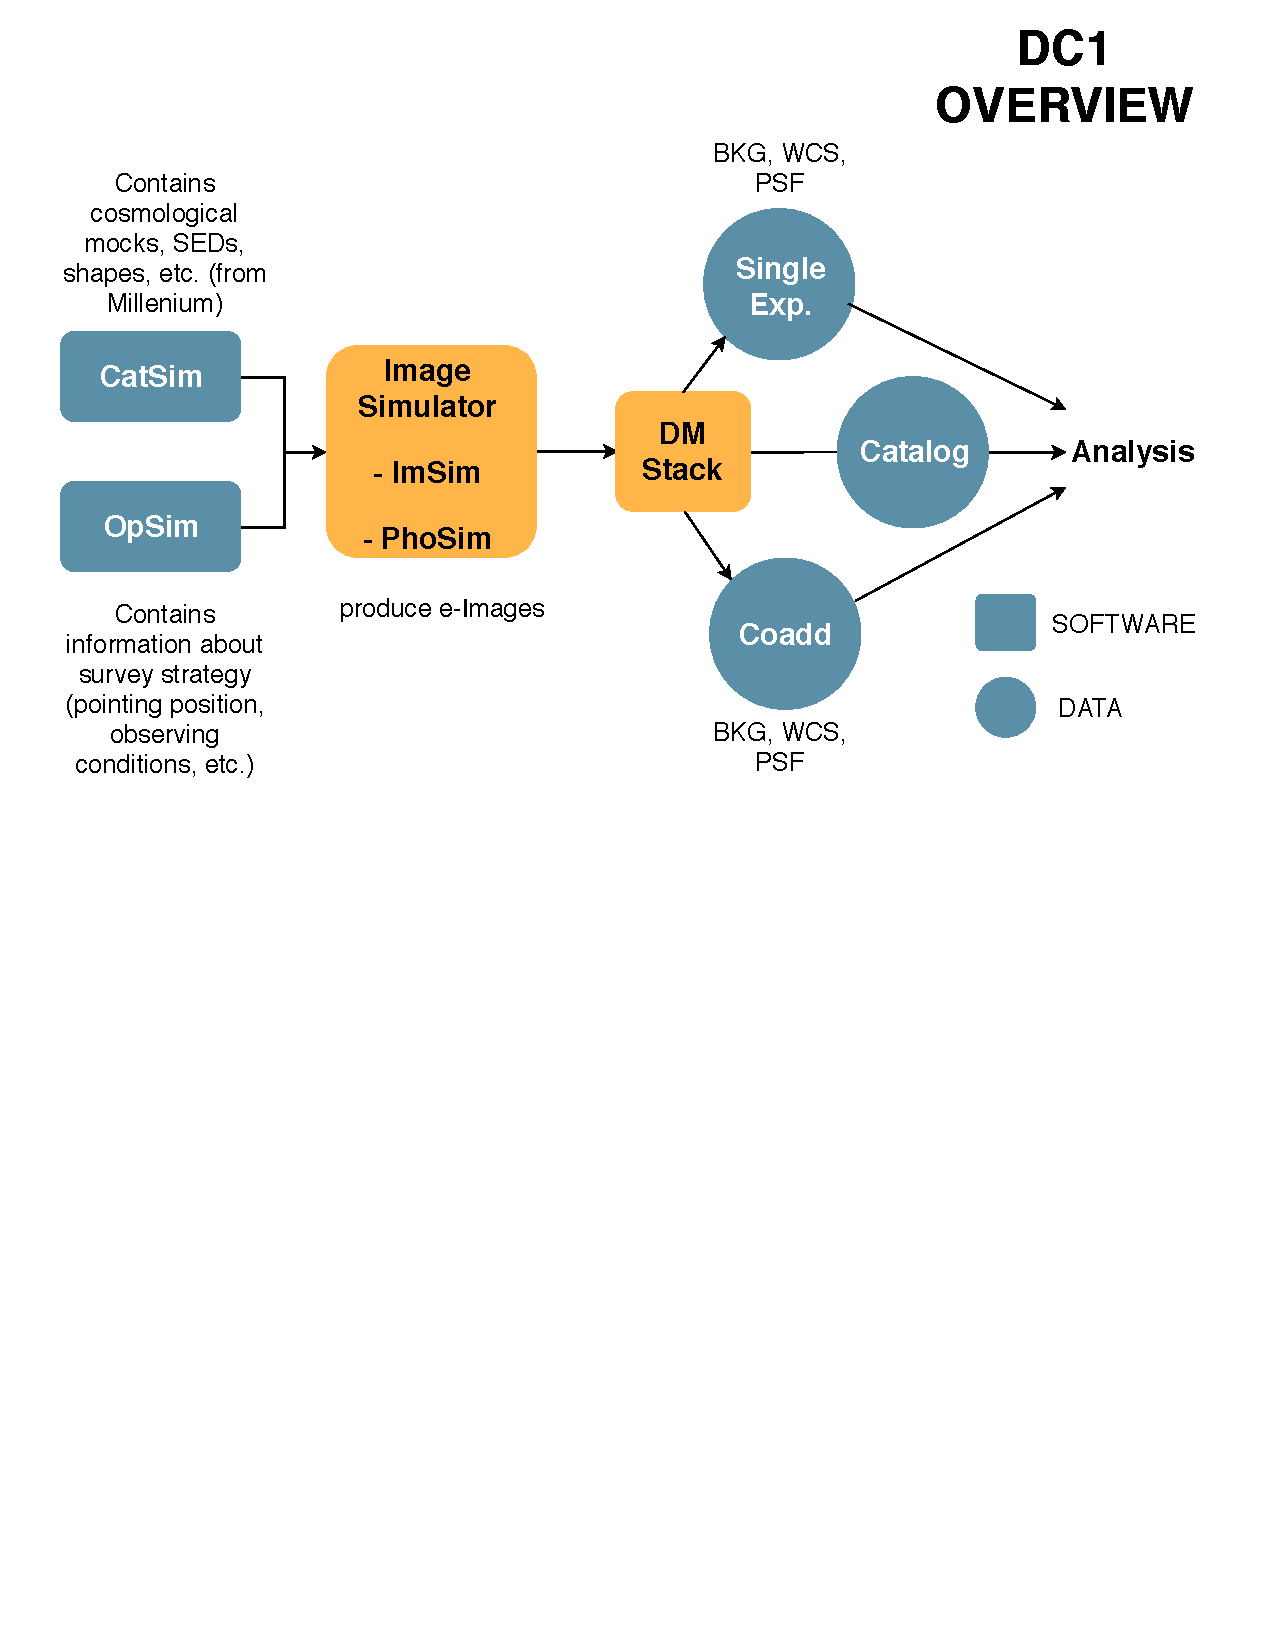
\includegraphics[trim={0cm 1.5cm 0cm 1.05cm}, clip, width=1.0\columnwidth]{dc1_workflow}
\caption{Workflow diagram for full data simulations. The image simulation step produces synthetic raw observations from a known truth catalog based on N-body simulations and simulated observing conditions. These data are processed by the LSST Science Pipelines to first generate calibrated single exposure images. These are calibrated both astrometrically and photometrically and are fed again into the LSST Science Pipelines that produce the image co-adds and a catalog of detected static sources. 
}

\label{fig:dc1_workflow}
\end{figure}


\subsection{Image generation: input catalog}
\label{sec:inputs}
Image simulations allow us to assess the detection and deblending performance of a given image-processing pipeline. For example, if we produce images using an object catalog with random positions uniformly distributed across the sky, as well as uniformly random shapes and fluxes, we can get information about detection efficiencies as a function of flux. However, the effects of source blending may not be realistic as we will not be able capture some correlations present in real data. On the other hand, using N-body simulations as the input to generate artificial images allows us to study all the aforementioned effects. We used the CatSim~\citep{2010SPIE.7738E..1OC,2014SPIE.9150E..14C} catalog as our input to account for these effects, and to be able to test our analysis pipelines. CatSim is a set of simulations provided by the LSST Simulations Team representing a realistic distribution of both Milky Way and extra-galactic sources. In particular, the extra-galactic catalog contains galaxies covering the redshift range $0 < z < 6$ in a 4.5$\times$4.5 degree footprint. The magnitude and redshift distributions are shown in \figref{catalog_plots}. The galaxies are generated by populating the dark matter haloes from the Millennium simulation~\citep{2005Nature.435.629S} using a semi-analytic baryon model described in \citet{2006MNRAS.366..499D} including magnitudes BVRIK, LSST-ugrizy, and bulge-to-disk ratios. For all sources, a spectral energy distribution (SED), is fit to the galaxy colors using \citet{2003MNRAS.344.1000B} spectral synthesis models. Fits are undertaken independently for the bulge and disk and include inclination dependent reddening. Morphologies are modeled using two S\'{e}rsic profiles~\citep{1963BAAA....6...41S} and a single point source (for the AGN). Half-light radii for the bulge components are derived from the absolute-magnitude vs half-light radius relation given by \citet{2011A&A...534A...3G}. Stars are represented as point sources and are drawn from the Galfast model~\citep{2008ApJ...673..864J}. More information about these catalogs can be found at the LSST Simulations webpage\footnote{\url{https://www.lsst.org/scientists/simulations/catsim}}.

\begin{figure}
\centering
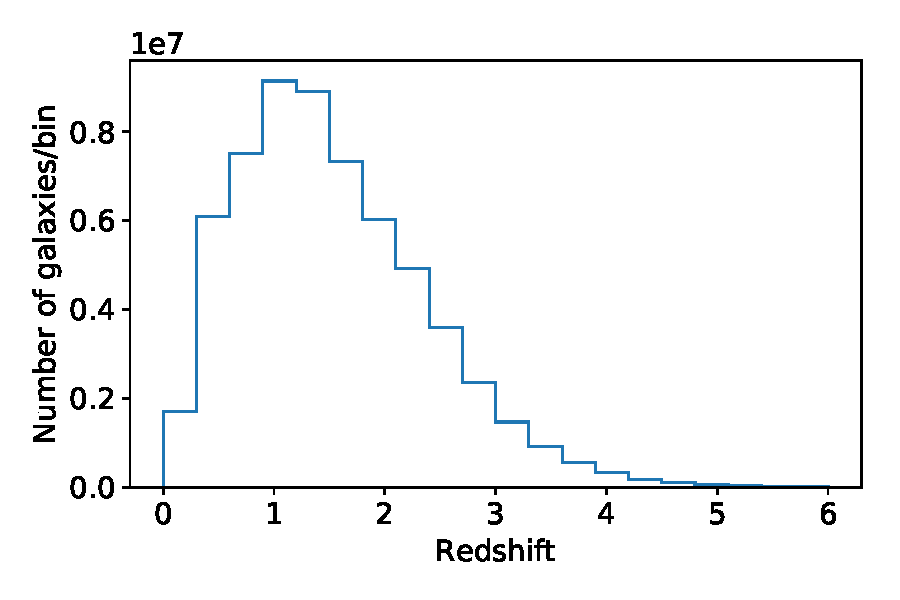
\includegraphics[width=0.9\columnwidth]{N_z_DC1.pdf}
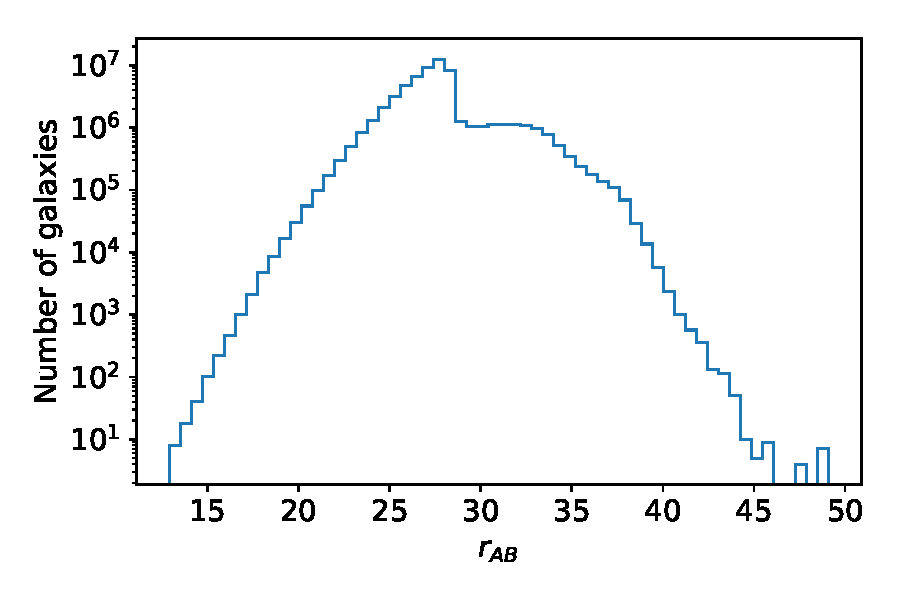
\includegraphics[width=0.9\columnwidth]{N_m_DC1.pdf}
\caption{Redshift (top) and magnitude (bottom) distribution for the galaxies used as inputs for the Data Challenge 1 simulations. In the magnitude distribution we include, as references, the typical depth for a single exposure (red dashed line) and the median depth in the deepest coadded DC1 simulation (black dashed-dotted line).}
\label{fig:catalog_plots}
\end{figure}


For DC1, we chose a nominal field centered at RA $\approx 93^{\circ}$ and Dec $\approx -29^{\circ}$. This field has a Galactic latitude of $b \approx -20^{\circ}$ and a dust extinction $0.05 \leq E(B-V) \leq 0.35$ and thus represents a typical region in the LSST wide-fast-deep survey~\citep{Overview}. The CatSim catalog was tiled to generate a $\sim 40$ deg$^{2}$ footprint covering 4 LSST full focal plane pointings. This approach introduces a periodicity that induces extra correlations in our sample, however, this is not a major issue as we are unable to measure correlations on relevant scales ($> 1$ deg.) with any useful precision.

\begin{figure}
\centering
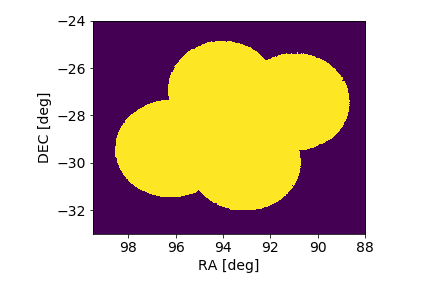
\includegraphics[width=0.9\columnwidth]{footprint.png}
\caption{Footprint of the DC1 dataset. We simulate 4 LSST full focal plane pointings which roughly corresponds to 40 deg$^{2}$.}
\label{fig:footprint}
\end{figure}

After tiling, the input catalog contains approximately $63.1$ million sources, of which 97\% are galaxies whose redshift and magnitude distributions are depicted in \figref{catalog_plots} and remaining objects are stars. We simulate $r$-band observation to the LSST full depth ($10$ years, 30-second exposures). The final footprint can be seen in \figref{footprint}. We simulate observations within this footprint using a simulated observing cadence generated with the LSST Operations Simulator (OpSim)~\citep{2014SPIE.9150E..15D}. In particular, we use the \texttt{minion\_1016}\footnote{\url{https://www.lsst.org/scientists/simulations/opsim/opsim-v335-benchmark-surveys}} database, which contains simulated pointing position, observation date and filter. It also contains information about simulated observing conditions, such as, seeing, sky brightness, moon position, etc. We use 4 pointings with $\approx 184$ visits per pointing over 10 years from this database for DC1.

\subsection{Dither strategy}
\label{sec:dithering}

As mentioned in \secref{design}, we use OpSim's output, which contains a realization of the LSST observing cadence and the survey footprint. Since OpSim divides the sky into hexagonal tiles, the nominal telescope pointings lead to overlapping regions across adjacent tiles that are observed more often than the non-overlapping part of the field-of-view (FOV), resulting in depth non-uniformity on the scale of $\sim$1 degree and consequently can introduce systematic uncertainties \citep{2016ApJ...829...50A}. In an effort to mitigate these effects, and following the same approach that will be taken with LSST data, we implement \textit{dithers} -- offsets in the nominal telescope pointings. Specifically, here we use \textit{large}, i.e., as large as the FOV, random translational dithers, implemented after every visit, and random rotational dithers implemented after every visit. The specific translational dither strategy is chosen based on a more extensive study of the various (translational) dither strategies in \citet{2016ApJ...829...50A}, where random dithers after every visit are found to be amongst the most effective.

For our purposes, we consider both an undithered and a dithered observing strategy. For the dithered strategy, some visits will contain sensors that fall outside of the DC1 region; these sensors were not simulated in order to save computational resources. However, the sensors that partially overlapped our nominal field of view were simulated. In total, we simulate $\approx 184600$ sensor/visits for the dithered simulation and $\approx 151000$ for the undithered simulation.




\section{Image generation and processing}
\label{sec:image_generation_pipeline}
% ---------------------------------------------------------------------

The artificial generation of astronomical images is a complex and computationally demanding process. In recent
years, there have been major efforts in the community to create software that enables the generation of astronomical images, with various choices made in terms of level of complexity, fidelity, and computational efficiency, such as \texttt{UFIG}~\citep{2016ApJ...817...25B}, and PhoSim~\citep{2015ApJS..218...14P}. In our case, we model the input sources using
two independent approaches. 

Firstly, we use PhoSim, a fast photon Monte Carlo code that enables the generation of images with a high level of realism. We use PhoSim version 3.6 with a custom configuration\footnote{\url{https://github.com/LSSTDESC/SSim_DC1/issues/27}} that enables some
approximations (photon-bundling) to be made when generating the sky background in order to reduce the overall computing time needed to produce the images.

We also employ imSim\footnote{\url{https://github.com/LSSTDESC/imSim}} (Walter et al., {\em in prep.}), which internally uses GalSim~\citep{2015A&C....10..121R} as a library for image rendering, and uses LSST-specific information (e.g., the geometry of the CCDs and the focal plane, the system throughputs in the different bands, etc.) to generate LSST-like images. For this simulation campaign we use an early pre-release version of imSim, version \texttt{v.0.1.0}, which performs a series of approximations that allow us to complete the image simulations significantly faster ($\sim 60\times$) than PhoSim, at the expense of a loss in realism. These approximations include simplifications in the PSF model (PhoSim performs ray-tracing through the atmosphere, while this version of imSim uses simple parametric models for the PSF) and lack of sensor effects, which were deemed acceptable given the goals of DC1.

Due to the computational resources needed to run PhoSim we could only generate one campaign of the dithered DC1-PhoSim data, whereas we could produce the dithered and undithered campaigns for imSim. Furthermore, comparison of the results for the PhoSim and imSim images has proven less informative than intended due to some unusual features of unknown origin in the sky backgrounds in the PhoSim images\footnote{Several aspects of the implementation of the sky background rendering -- including the photon-bundling approximations -- are updated in subsequent versions of PhoSim, so this finding may not carry over to later PhoSim versions.}. For these reasons, we focus on the analysis and comparison of dithered versus undithered imSim images for the rest of this work.

\subsection{imSim}
\label{sec:imsim_pipeline}

imSim is an open-source image simulation software package that uses GalSim. It allows the user to change the level of realism of the simulations, by increasing the complexity of the PSF, background and source modeling. In particular, we use a pre-release version specifically meant to perform the DC1 simulations: imSim \texttt{v.0.1.0}\footnote{\url{https://github.com/LSSTDESC/imSim/releases/tag/0.1.0}}.


For DC1, we simulate each CCD of the focal plane individually, and generate a single image with a 30-second exposure time to simplify data handling. We omit instrumental effects and variability in the optical model across the focal plane. Since this is the first DESC data challenge, we want to ensure that we are able to generate and process the simplest cases, and then, building upon this base, increase the complexity and level of realism for future data challenges. Our sky brightness model is based on the \citet{1991PASP..103.1033K} model provided by OpSim, refined by the detailed wavelength dependence of the phenomenological model from~\citet{2016SPIE.9910E..1AY}. The PSF model is a Gaussian for the system (telescope, CCD and other elements that may be in the optical path different than the atmosphere) with a full-width half-maximum airmass, $X$, dependence, $\mathrm{FWHM_{sys}} = 0.4" X^{0.6}$, to mimic the degradation in the image quality due to, e.g., gravity load\footnote{See LSE-30~\url{http://ls.st/lse-30} p.~80}. A Kolmogorov profile\footnote{\url{http://galsim-developers.github.io/GalSim/_build/html/_modules/galsim/kolmogorov.html}} is used to model the atmosphere which is also airmass dependent. The airmass, $X$, depends on the angular distance to the zenith, $Z$, as follows~\citep{1991PASP..103.1033K}:

\begin{equation}
X = (1 - 0.96\sin^{2}{Z})^{-0.5}.
\end{equation}
For DC1, imSim can generate three different types of objects: stars, which are modeled as PSF-like objects; galaxies, which are modeled as composite (bulge plus disk) S\'{e}rsic profiles~\citep{1963BAAA....6...41S} using
the parameters given by CatSim; and AGNs which are also modeled as point sources and, for simplicity, without any variability. Newer versions of imSim have the ability to generate more complex galaxy morphologies (e.g., they can include random Gaussian knots). The brightness for these sources is computed using the magnitudes from CatSim, which are converted to counts using the latest version of the LSST throughputs\footnote{\url{https://github.com/lsst/throughputs}}. In DC1, we clip the objects at magnitude 10 in order to improve the computational efficiency. Saturation is emulated by clipping the maximum number of counts per pixel at 100,000.

The final products of this pipeline are FITS images with information about the observing conditions contained in the header. We generated more than 300,000 images in total (including both the \textit{dithered}, and \textit{undithered} fields). The average time to simulate each CCD is $\sim 4300$ seconds and the total production time is $\sim 270,000$ CPU-hours.

\subsection{Image processing}
\label{sec:image_processing_pipeline}

The outputs of these simulations are processed using the LSST Science Pipelines~\citep{Overview,ScienceBook,WhitePaper,2015arXiv151207914J,2018PASJ...70S...5B} using version 13.0\footnote{\url{https://pipelines.lsst.io/releases/v13_0.html}}, which we will refer to as the DM stack. The DM stack is an open-source, high-performance data processing and analysis system intended for use in optical and infrared survey data. The code can be found at \url{dm.lsst.org} and \url{pipelines.lsst.io}. A brief schematic of some of the steps in the image processing pipeline can be seen in \figref{dc1_workflow} as green squares. The raw, uncalibrated single exposures are used as inputs. The software performs the reduction, detection, deblending and measurement on individual visits. It then combines the single-visit images to produce the so-called coadds. This is done by computing a weighted average of resampled overlapping sensor images. For more information about this process, see Section 3.3 in~\citet{2018PASJ...70S...5B}. After assembling the coadd images, the DM stack performs measurements on them producing a catalog. The DM stack provides calibrated images and source catalogs for the individual visits and coadds stored in \texttt{FITS} files. In total, we detect and measure $\sim 10.6$ (9.7 for the undithered simulation) million objects with position, flux and shape information. We activated optional extensions for the pipeline to include \texttt{CMODEL} fluxes (see \cite{2018PASJ...70S...5B} for more details) and \texttt{HSM} shapes~\citep{2003MNRAS.343..459H,2005MNRAS.361.1287M}. An example coadd cutout is shown in \figref{coadd_example}.

The reduction pipeline is essentially the same as for HSC~\citep{2018PASJ...70S...5B}. This is going to allow us to use the HSC selection criteria as basis for our analysis, and can potentially enable direct comparisons between datasets for further validation.

\begin{figure*}
\centering
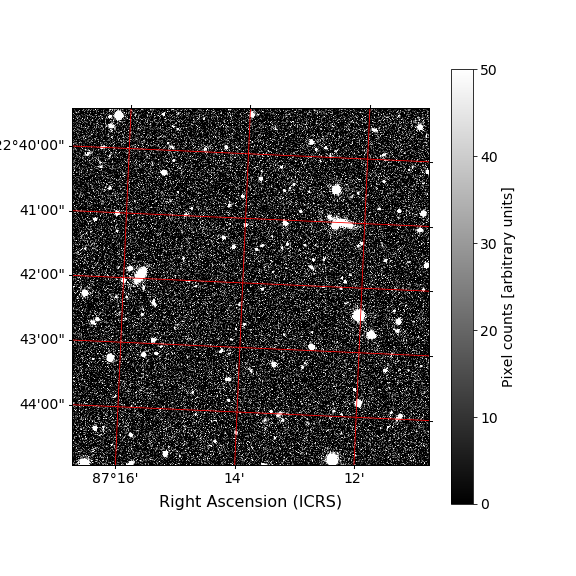
\includegraphics[width=0.4\textwidth]{calexp_example.png}
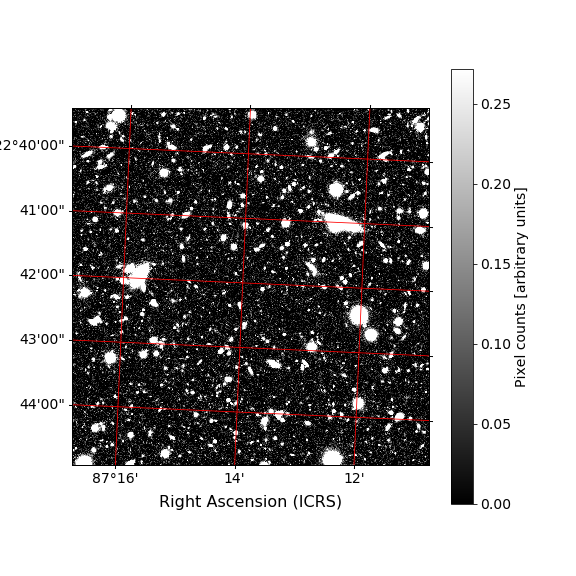
\includegraphics[width=0.4\textwidth]{coadd_example.png}
\caption{Example of a 1000 $\times$ 1000 pixel cutout from a calibrated exposure (left), i.e. background subtracted, reduced single-epoch image; and a full depth coadd (right). We can see the stark difference in the number of objects that are detectable by eye.}
\label{fig:coadd_example}
\end{figure*}

The total processing time for our data is $\approx 29,000$ CPU-hours.

\section{Matching inputs and outputs}
\label{sec:matching}

Using end-to-end simulations, one can potentially trace each measured photon to its corresponding source and fully characterize the image generation and measurement processes. In practice, this is very difficult due to the large data volume and the fact that the data reduction pipeline is built around pixelated images rather than tagged photon counts.

Nevertheless, the output catalog is a noisy representation of the underlying true catalog and we need to find a way to connect the two. 
The simplest way to connect two catalogs is by using the positions of the objects in the sky. This approach has been extensively used in the literature~\citep{1977A&AS...28..211D,1983Obs...103..150B,1986MNRAS.223..279W} and performs reasonably well when blending is low (i.e, when there are few overlapping sources in the image). However, when the blending fraction is high, this approach might be not be sufficient. In this case, matching other quantities like flux, color and/or shape can become useful~\citep{2008ApJ...679..301B, doi:10.1146/annurev-statistics-010814-020231}. However, when adding other quantities, the matching process can become slower and result in a lower matching completeness. For more details about challenges relating two different catalogs, we refer the reader to~\citet{doi:10.1146/annurev-statistics-010814-020231}. 

We compare two different matching strategies: positional matching, where we find the objects in the truth catalog closest to the detected objects, which we will refer to as \textit{pure spatial matching} and will denote as \textsf{S}; and positional matching with magnitude matching, which we will refer to as \textit{spatial+magnitude matching} and denote as \textsf{S+M}, where for each detected object we find objects from the input catalog that lie within a three pixel radius ($0.6 \arcsec$). After this, we select the object that is closest in magnitude as long as the difference in r-band magnitude, $\Delta r$, is less than a certain threshold. In our case, we conservatively choose $|\Delta r| < 1.0$. Using this approach, if none of the neighbors fulfill these conditions, the detected source is considered unmatched. Note that in the case of pure spatial matching all sources are matched to an object in the true catalog.

In both cases, we build a \texttt{KDTree}~\citep{scikit-learn} using the positions of detected objects flagged with \texttt{detect\_isPrimary=True} which ensures that the source has been fully deblended and was detected in the inner part of the coadd regions (see~\citet{2018PASJ...70S...5B} and ~\citet{2018PASJ...70S..25M} for more details). In order to speed up the processing and to reduce the usage of computational resources we build the \texttt{KDTree} using output sources from 30 randomly selected coadd regions (patches) in the dithered simulation (the undithered simulation yields the same results and conclusions) containing 975,605 detected sources fulfilling the aforementioned condition (we will refer to these as primary outputs or primary detected sources). Using this sample, we find that 95.2\% of these sources are matched using the spatial+magnitude matching (by construction all of them are matched using the pure spatial matching approach). One interesting metric is the fraction of primary detected sources that have been matched to the same object in the input catalog, which we will denote as $f_{\mathrm{multi}}$. This is an unusual occurrence, but can occur when a noise fluctuation is marked as a source; this fluctuation is a primary detected source but has no counterpart in the input catalog. Another example are bright objects that have been shredded and are detected as several fainter sources. We find that these kind of matches are $\sim 100$ times more likely to happen using the pure spatial matching ($f_{\mathrm{multi}} = 3 \times 10^{-3}$) than in the spatial+magnitude matching ($ f_{\mathrm{multi}} = 2 \times 10^{-5}$). This is expected because, in the cases where the primary detected source is a random fluctuation or a shredded source, it is unlikely that the measured flux is close to the flux of a neighboring source thus producing an unmatched source in the case of using spatial+magnitude matching. We also find that both approaches select the same best matching source in the input catalog for only 68\% of the primary detected sources for which we found a suitable match. These differences can be due to several reasons, e.g. objects with a poorly determined centroid position that are close to other objects in the input catalog (remember that the input catalog contains objects up to $r=28$), objects with poorly determined fluxes (low SNR), etc.

We also compare the photometric residuals, $\Delta r = $ \texttt{CMODEL} - $r_{true}$ (i.e. measured - input), using both approaches in~\figref{matching_comparison}. The resulting median photometric residual seems strongly biased in the case of using just pure spatial matching, and the scatter is very large as shown by the error-bars. However, in the case of spatial+magnitude matching, the median residuals and their error-bars are smaller, as expected given the maximum magnitude threshold. We can see that in this case the biases are still significant, partially due to the fact that we are only going to be able to measure objects where the noise contributes to make it brighter, and we lose the objects that fluctuate to dimmer fluxes/magnitudes, biasing the overall residual distribution. On top of that, the presence of spurious matches also contributes to this effect. This can be mitigated using a smaller tolerance in magnitude (for example using 0.5 mag instead of 1 mag) but that implies an overall reduction of the number of matched primary detected sources. Finally, observing the magnitude difference between inputs and outputs of individual matched sources using the spatial+magnitude technique, we can see that this distribution is centered around zero, except for very bright sources ($r < 17$), where saturation prevents us from having an accurate determination of the fluxes. 

\begin{figure}
\centering
%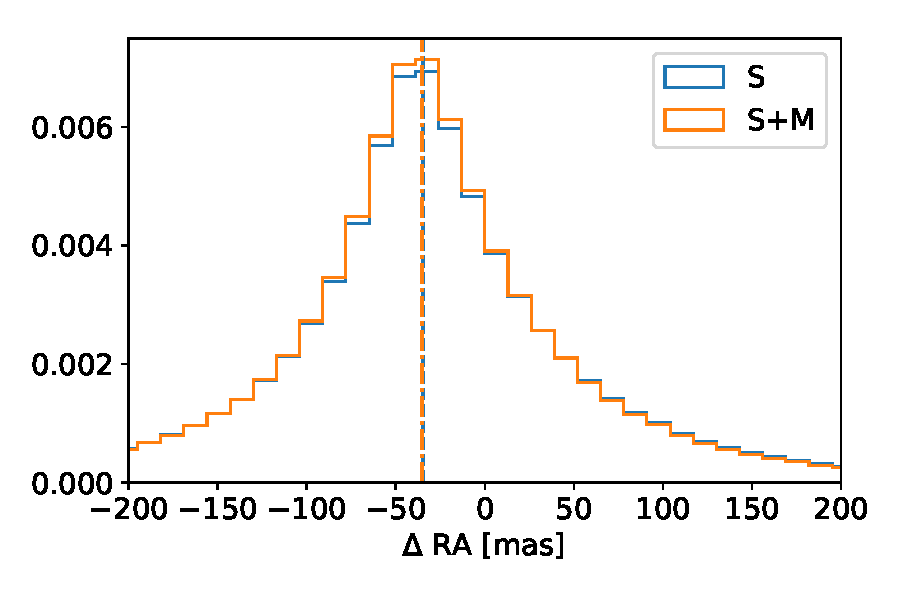
\includegraphics[width=0.85\columnwidth]{astrometry_residual_comparison}
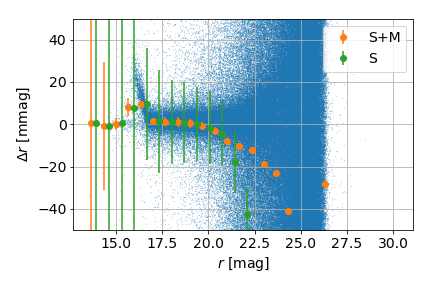
\includegraphics[width=0.85\columnwidth]{photometry_residual_comparison}
\caption{Top: Normalized distribution of measured astrometric residuals (in the RA axis but similar results are found for the Dec. axis) for pure spatial matching (blue) and spatial+magnitude matching (orange), the median values of each distribution are marked by dashed lines and dashed-dotted lines respectively. Bottom: Median per-bin photometric residual as a function of measured magnitude for pure spatial matching (green), and spatial+magnitude matching (orange) using 30 magnitude bins between $r$-band magnitude 10 and 30. We also show the individual residuals for the matched objects using spatial+magnitude matching (blue dots).}
\label{fig:matching_comparison}
\end{figure}

Different matching techniques have different potential applications and strengths~\citep{doi:10.1146/annurev-statistics-010814-020231}. In our case, we want to use these matching techniques to provide a clean (flux-limited) sample to perform two-point clustering analyses. Given that magnitude precision and accuracy will be important for our sample selection, the \textbf{spatial+magnitude} matching technique will be sufficient to clean the sample from artifacts and poorly measured sources. However, more complicated matching techniques may be necessary for other use cases.
 
 
\section{Output catalogs and validation}
\label{sec:catalogs}
%\subsection{Output Catalogs}
After being processed, the catalogs are stored at the National Energy Research Scientific Computing Center (NERSC)\footnote{\url{http://www.nersc.gov}} and accessible to DESC collaborators. We generate \texttt{pandas
DataFrames}~\citep{mckinney-proc-scipy-2010} and databases for each one of the coadds and input catalogs, providing collaborators some flexibility in data access for their own analyses. As mentioned earlier, the output catalogs contain 10.6 million objects (9.7 million in the undithered case) covering an area
of $\sim$43 deg$^{2}$. The catalogs include information about position, size, shape and magnitude for every object. They also include several flags that give information about the presence of interpolated/saturated pixels in the objects and whether or not these objects are close to the edge of a CCD.

\subsection{LSST Science Requirements Document Key Performance Metrics and DESC Science Requirements Document}

In order to check the level of realism and the accuracy of the processed catalogs we perform several quality assurance tests. These tests check two different aspects: the level of realism and consistency of the simulations, and the performance of the processing pipeline. The results in this section are presented for the dithered simulation, however, unless stated, the procedures and behavior are similar for the undithered simulation.

Firstly, we perform some basic sanity checks and, after this, we process the output individual-visit catalogs through the LSST Project package \texttt{validate\_drp}\footnote{\url{dmtn-0008.lsst.io}, \url{https://github.com/lsst/validate_drp}}.
The \texttt{validate\_drp} package calculates the Key Performance Metrics (KPMs) from the LSST Science Requirements Document\footnote{\url{https://ls.st/LPM-17}}~\citep{LPM-17}, which we will refer to as the LSST-SRD. This document describes science-driven requirements for LSST data products and we use it as a guide to check the status of our end-to-end pipeline, with a special focus on the performance of the processing pipeline. In particular, we will use the LSST-SRD version 11 throughout this work. For quick reference, a brief description of the requirements from the LSST-SRD studied in this section can be found in Appendix~\ref{app:lsst_srd}. In addition, we also validate our dataset using some of the requirements in the DESC Science Requirement Document~\citep[][DESC-SRD;]{2018arXiv180901669T}, which we will refer to as DESC-SRD.
 
By design, our simulations do not satisfy some of the requirements in the LSST-SRD, such as the number of filters in the surveyed fields (Filter complement in \tabref{kpm_table}) or the number of filters (Nfilt) used in a given night because we only simulate images in $r$-band. On the other hand, our images automatically meet some criteria due to the design choices, e.g., requirements about the pixel size since it is fixed. However, some requirements in both the LSST-SRD and the DESC-SRD cannot be tested with these single-band images (for example, KPMs involving colors) and we will ignore such tests in this work.

The results of {\bf these checks are summarized in \tabref{kpm_table}}. We proceed now to provide a description of these tests. More details about these tests and their motivation can be found in both the LSST-SRD~\citep{LPM-17} and the DESC-SRD~\citep{2018arXiv180901669T}.
\begin{table*}
\begin{tabular}{|c|c|c|c|c|c|}
\hline
KPM/Requirement & Pass/Fail Criterion & DC1 test result & Passed & Section & Figure(s)\\
%\hline
%Filter complement & ugrizy & r & \textcolor{blue}{N} & & \\
%Nfilters & 3 & 1 & \textcolor{blue}{N} & & \\
%Nv1 & 184 & 184 & \textcolor{blue}{Y} & &\\
%pixSize (arcsec) & 0.22 & 0.2 & \textcolor{blue}{Y} & &\\
\hline
AA1 (milliarcsec) & 100 & 20 & Y & \ref{sssec:astrometry} & \ref{fig:AA1} \\
AM1 (milliarcsec) & 20 & 8 & Y  & & \ref{fig:validate_drp_AMx}\\
AF1 (\%) & 20 & 13 & Y &  & \ref{fig:validate_drp_AMx}\\
%AD1 (milliarcsec) & 40 & - & -  &  & \ref{fig:validate_drp_AMx}\\
AM2 (milliarcsec) & 20 & 4 & Y  &  & \ref{fig:validate_drp_AMx}\\
AF2 (\%) & 20 & 9 & Y  &  & \ref{fig:validate_drp_AMx}\\
%AD2 (milliarcsec) & 40 & - & -  &  & \ref{fig:validate_drp_AMx}\\
AM3 (milliarcsec) & 30 & 7 & Y  &  & \ref{fig:validate_drp_AMx}\\
AF3 (\%) & 20 & 2 & Y  &  & \ref{fig:validate_drp_AMx}\\
%AD3 (milliarcsec) & 50 & - & -  &  & \ref{fig:validate_drp_AMx}\\
\hline
PA1 (millimag) & 8 & 6 & Y  & \ref{sssec:photometry} & \ref{fig:validate_drp_PA1}\\
PF1 (\%) & 20 & 17 & Y  &  & \ref{fig:validate_drp_PA1}\\
%PA2 (millimag) & 15 & - & -  &  & \ref{fig:validate_drp_PA1}\\
\hline
PA3 (millimag) & 15 & 0.06  & Y  & \ref{sssec:zeropoints} & \ref{fig:PA34}\\
PF2 (\%) & 20 & 0 & Y  &  & \ref{fig:PA34}\\
%PA4 (millimag) & 20 & - & -  & & \ref{fig:PA34}\\
%PA5 (millimag) & 10 & 1.4 & check\\
PA6 (millimag) & 20 & 17 & Y  &  & \ref{fig:PA34}\\
\hline
%%%Fleak (\%) & 0.02 & 0 & \textcolor{blue}{Y}\\
%%%FleakTot (\%) & 0.1 & 0 & \textcolor{blue}{Y}\\
D1 (mag) & 24.3 & 24.3 & Y & \ref{sssec:depth} & \ref{fig:DF1_checks}\\
%DF1 (\%) & 20 & - & - & & \ref{fig:DF1_checks}\\
Z1 (mag) & 24.0 & 24.1 & Y & & \ref{fig:DF1_checks}\\
DB1 (mag/r-band) & 24.3 & 24.3 & Y &  & \ref{fig:DF1_checks}\\
%DF2 (\%) & 20 & - & - &  &  \\
Z2 (mag) & 0.4 & 0.1 & Y &  & \\
\hline
%%%S1 (0.44) & 0.59 & check & check\\
%%%S1 (0.60) & 0.72 & check & check\\
%%%S1 (0.80) & 0.89 & check & check\\
%%%SF1 (\%) & 10 & check & check\\
%%%SX & 1.2 & check & check\\
%%%SXE & 0.59 & check & check\\
SE1 & 0.04 & 0.001 & Y & \ref{sssec:psf} & \ref{fig:SE1_DC1}\\
%EF1 & 10 & - & - &  &\\
SE2 & 0.1 & 0.002 & Y & & \ref{fig:SE1_DC1}\\
SR1 (arcsec) & 0.80 & 0.64 & Y & & \\
SR2 (arcsec) & 1.31 & 1.01 & Y & & \\
SR3 (arcsec) & 1.81 & 1.79 & Y & &\\
TE1 & $3 \times 10^{-5}$ & $3\times 10^{-6}$ & Y & & \ref{fig:TEx}\\
TE2 & $3 \times 10^{-7}$ & $9\times 10^{-8}$ & Y & & \ref{fig:TEx}\\
\hline
WL4-Y10 (\%) & 0.1 & 0.05 & Y & & \ref{fig:WL4-Y10}\\
%%%TEF & 15\% & - & -\\
%%%TE3 & $6 \times 10^{-5}$ & - & N\\
%%%TE4 & $5 \times 10^{-7}$ & - & N\\
%%%\hline
\end{tabular}
\caption{Summary of Key Performance Metrics (KPMs) and DESC-SRD requirements that we check to test the quality of our end-to-end pipeline. The criteria that are fixed due to design choices are shown in blue.} %We mark with dashes the quantities that we use as auxiliary to compute some of the criteria, e.g., we use EF1 to compute SE2.}
\label{tab:kpm_table}
\end{table*}

\subsubsection{Astrometric performance}
\label{sssec:astrometry}
We start by checking the absolute astrometry by comparing the input and output catalogs in~\figref{AA1}. This test helps us determine if the galaxies are generated in the correct position in the sky, and if our pipeline is able to accurately and precisely reconstruct the position of the simulated objects. A precise astrometric solution is necessary in order to compute unbiased clustering statistics, given that they mostly depend on the separation between objects. We find a mean (and median) deviation of 38 milliarcseconds between the input and measured positions. This is due to the fact that the corrections for proper motion were not present in the version \texttt{13.0} of the DM stack. However, this bias is still below the minimum specifications for the absolute astrometric performance of LSST as defined by the LSST-SRD, which is 100 milliarcseconds, and is driven mainly by orbital computations of solar system objects~\citep{LPM-17}. 

\begin{figure}
\centering
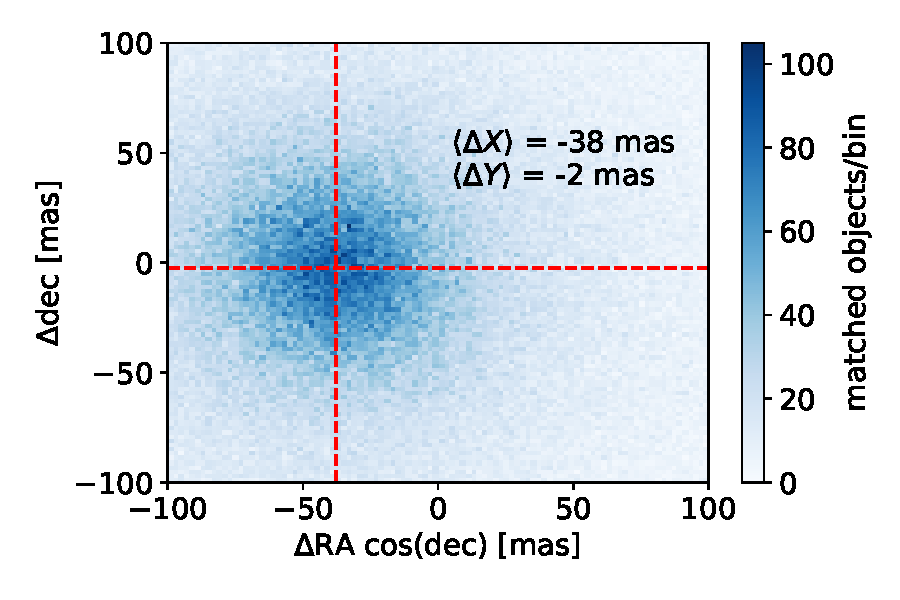
\includegraphics[width=0.9\columnwidth]{astrometric_residuals_single_visit_2d}
\caption{Astrometric residuals when comparing with the input catalogs for 500 randomly selected visits in the dithered simulation. We find a bias of 38 milliarcseconds in the measured right ascension due to uncorrected proper motion. We obtain similar results using the undithered simulation.}
\label{fig:AA1}
\end{figure}

We now focus on checking the astrometric repeatability in~\figref{validate_drp_AMx}. We check that the positions and distances between objects are consistent among different visits, this way, we will obtain consistent clustering results. We compute the RMS of the separation between pairs of stars separated by $D=5, 20$ and $200$ arcmin, obtaining AM1=8 mas, AM2=4 mas and AM3=7 mas. We check that no more than AF1=AF2=20\% (AF3=30\% in case of $D=200$ arcmin) of these pairs deviate more than 40 mas (50 mas for $D=200$ arcmin) from the median.

\begin{figure}
\centering
\includegraphics[width=0.9\columnwidth]{{DC1-imsim-dithered_r_validate_drp.AM1_D_5_arcmin_17.0_21.5_mag}.png}
\includegraphics[width=0.9\columnwidth]{{DC1-imsim-dithered_r_validate_drp.AM2_D_20_arcmin_17.0_21.5_mag}.png}
\includegraphics[width=0.9\columnwidth]{{DC1-imsim-dithered_r_validate_drp.AM3_D_200_arcmin_17.0_21.5_mag}.png}
\caption{
Astrometric repeatability: variation in distances measurement between pairs of stars at (top) 4-6$\arcmin$, (middle) 19-21$\arcmin$, (bottom) 199-201$\arcmin$.  AM(1,2,3) are the distance measurements, while AF(1,2,3) are the fraction of pairs lying outside the a specified limit AD(1,2,3).
The performance is excellent, with characteristic values all below the LSST-SRD levels.}
\label{fig:validate_drp_AMx}
\end{figure}

We find that our dataset pass all of these astrometric requirements, guaranteeing that the positions will be useful for clustering analyses. Note that for future versions of the LSST science pipeline, the overall astrometric repeatability will improve with the refinements of the PSF modeling under development. 

\subsubsection{Photometric performance}
\label{sssec:photometry}
Accurate and consistent photometry is important in order to have a robust flux limited sample, and well behaved photometric redshifts. This is why we also validate the photometric repeatability given by our processing pipeline by comparing the measured magnitude of bright (SNR $> 100$) point-like objects across different visits. This test validates that the pipeline is reconstructing fluxes of objects consistently across epochs, but also, that different epochs are produced consistently in our image simulations. The photometric repeatability (PA1) is 6~mmag as measured by the scaled interquartile range\footnote{IQR$\equiv$ 75th percentile minus 25th percentile, and then divided by the interquartile range of a Gaussian distribution with $\sigma=1$}, and 15.8~mmag as measured with the RMS; these distributions are shown in \figref{validate_drp_PA1}. The minimum specification is in the LSST-SRD is 8~mmag so our dataset and pipeline behave as required. The significantly greater RMS is dominated by a tail of scattered objects.%, see \figref{validate_drp_check_photometry}.

%We can separately look at the reported photometric uncertainty from the processing.  The Science Pipelines processing does not explicitly compare the reported photometric uncertainty to the per-epoch variation.  Thus comparing the quoted uncertainties to the observed variation of stars with no intrinsic variation validates the consistency between the pipeline calculations and the model outlined in \citet[][Eq. 4,5]{Overview}:
%\begin{eqnarray}
%\sigma^2 = \sigma^2_{\rm sys} + \sigma^2_{\rm rand}; \\
%\sigma^2_{\rm rand} = (0.04 - \gamma) &10^{0.4(m-m_5)} + \gamma 10^{0.8(m-m_5)};
%\label{eq:photometric_error}
%\end{eqnarray}
%where $\sigma$ is in magnitudes, $\gamma$ describes noise from the sky and detector electronics, and the 5-$\sigma$ point-source depth is given by:
%\begin{equation}
%\begin{split}
%m_5 = &C_m + 0.50 (m_{\rm sky} - 21~{\rm mag/{\rm arcsec}^2}) \\
%&+ 2.5 \log_{10} (0.7{\arcsec}/\theta_{\rm eff}) \\
%&+ 1.25 \log_{10} (t_{\rm vis} / 30~{\rm s}) - k_m (X-1);
%\label{eq:photometric_m5}
%\end{split}
%\end{equation}
%where $C_m$ summarizes the throughput of the telescope optics and camera, $m_{\rm sky}$ is the sky brightness, $\theta_{\rm eff}$ is the seeing, $t_{\rm vis}$ is the exposure time, $k_m$ is the airmass coefficient, and $X$ is the airmass. Note that the filter dependence is encoded in $C_{m}, m_{\rm sky}, \theta_{\rm eff}$, and $k_{m}$.

%Our fits find $m_5$ = 24.2~mag/arcsec$^2$ and $\gamma=0.038$ for $r$-band which are consistent with the \citet[][Table 2]{Overview} values of $m_5=24.35$~mag/arcsec$^2$, $\gamma=0.039$.  This demonstrates that we generate simulations of the telescope, detector, and sky in accordance with the \citet{Overview} estimates, as expected, since our inputs are based on these models.

%Note that we find $\sigma_{\rm sys}=0$~mmag, which is consistent with the idealized simulations we run for DC1 with no additional systematic sources of errors. 

We also check the fraction of photometric, bright point-like sources that deviate more than 15 mmag, finding only PF1=17\% over this threshold, in compliance with the requirements (PF1=20\%).

\begin{figure}
\centering
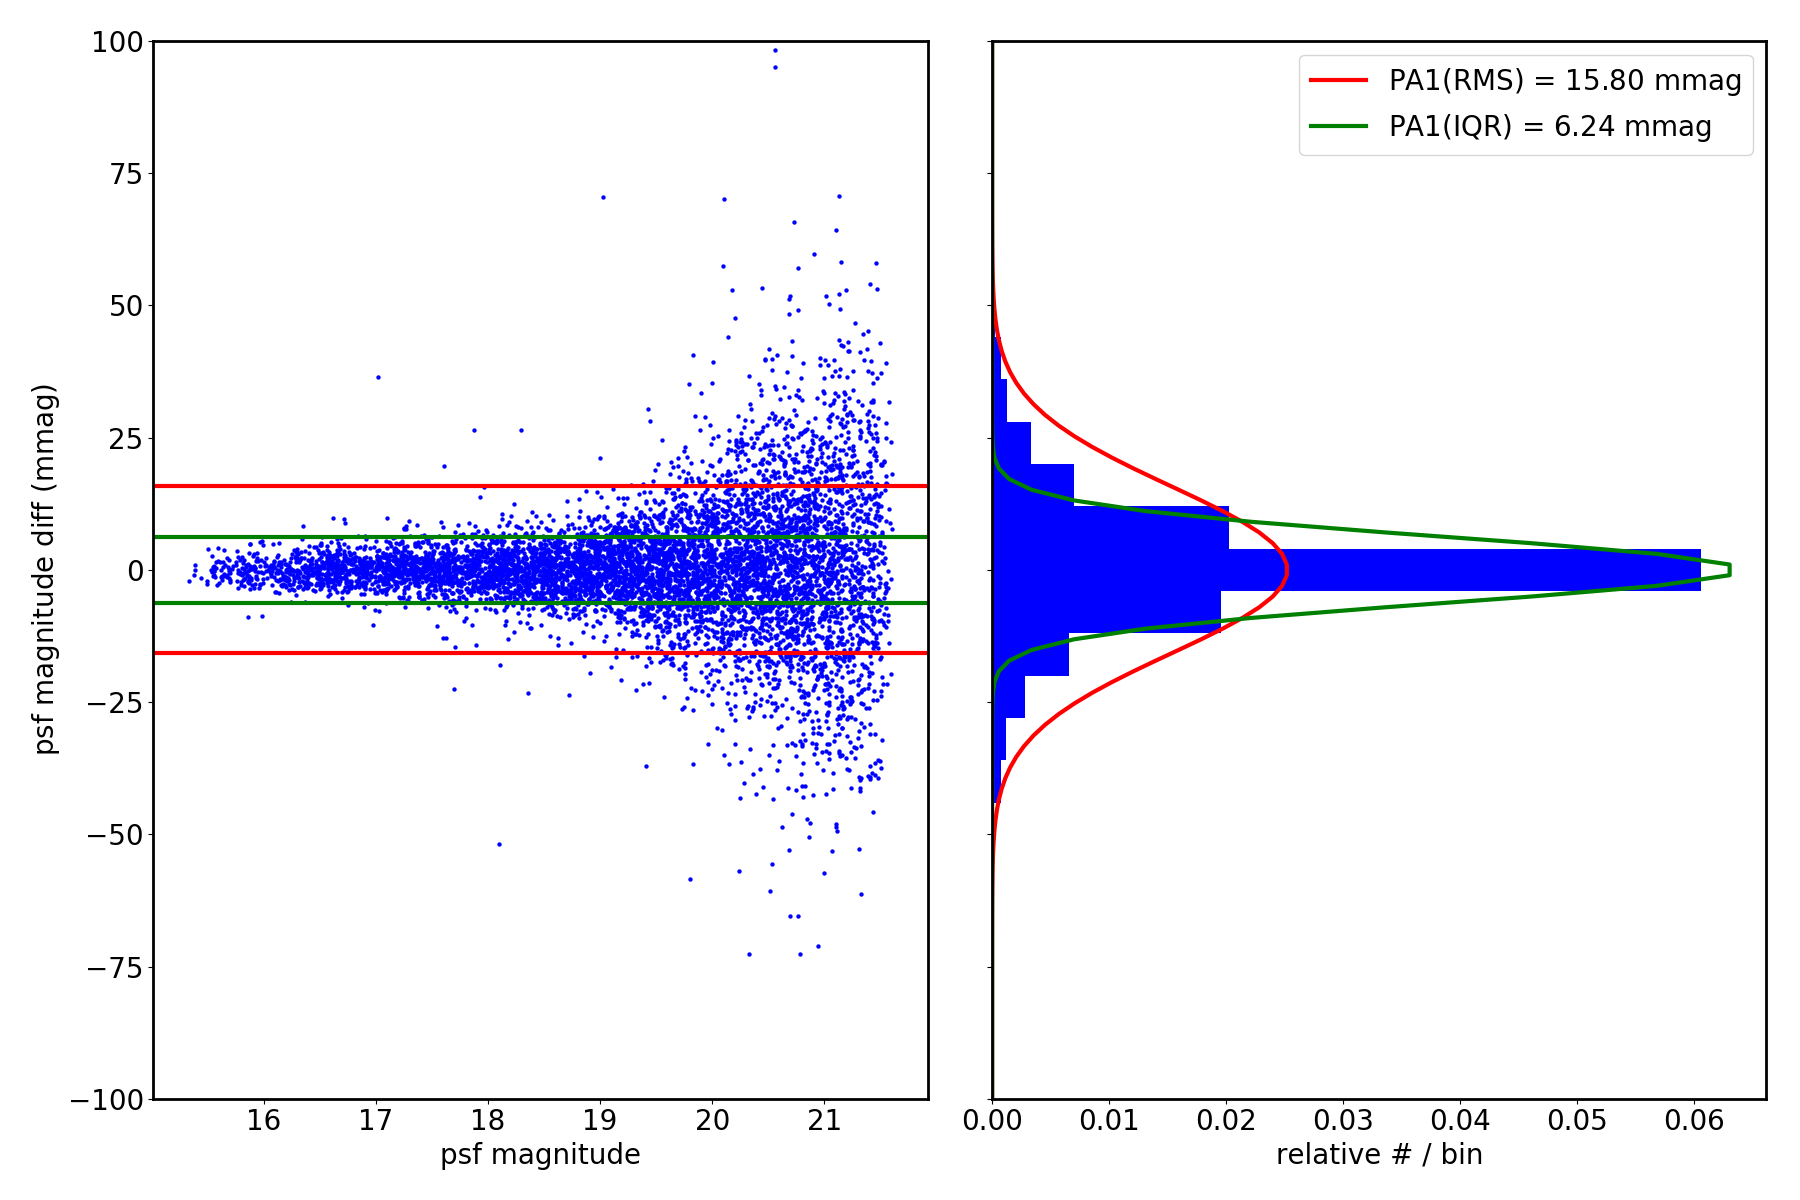
\includegraphics[width=0.9\columnwidth]{DC1-imsim-dithered_r_PA1.png}
\caption{(left) The magnitude difference of pairs of measurements of stars across visits for stars with a typical SNR $>100$.  (right) The histogram of these differences.  The Gaussian root mean square (RMS) is shown in red while the interquartile range is shown in green. Note that the distribution is more peaked than a Gaussian. The interquartile range (6.2~mmag) is {\em smaller} than the Gaussian RMS (15.8~mmag). This means that we have extended tails but most objects have very accurate magnitude measurements.}
\label{fig:validate_drp_PA1}
\end{figure}

%\begin{figure*}
%\centering
%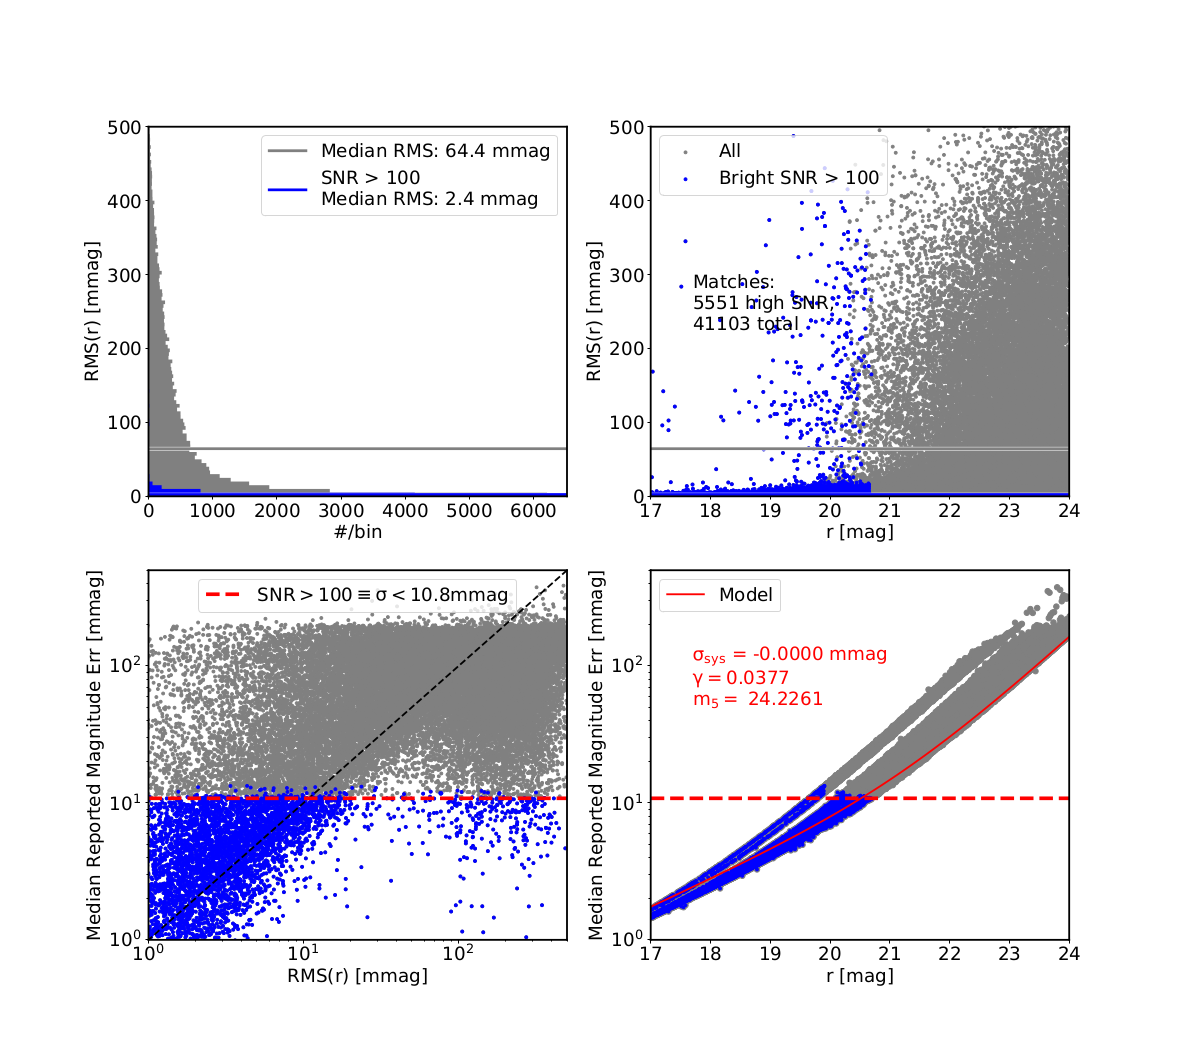
\includegraphics[width=1.6\columnwidth]{DC1-imsim-dithered_r_check_photometry.png}
%\caption{Photometric performance of the LSST DESC DC1.  (upper left) Horizontal histogram of the RMS distribution for each star for the full sample (grey) and ``bright'' sample (blue).  The blue sample is the same as that shown in Figure~\ref{fig:validate_drp_PA1}. Note that this RMS is the RMS of the measurements for a given star and so each entry in the histogram is one star. Thus, the median value here is 2.4~mmag, even thought the median of all RMS measurements in Figure~\ref{fig:validate_drp_PA1} was 15.8~mmag.  This difference is due to a population of objects that have a poor repeatability. (upper right) The RMS distribution as a function of magnitude of the star.  Here you can see the tight core of very repeatable measurements, along with a smaller population of objects with much higher scatter to their measurements. (lower left) Per-object median reported magnitude error by the pipeline versus the observed RMS over all of the measurements for an object.  Our $SNR>100$ cut is in the space of median reported error. (lower right) Per-object median pipeline-reported magnitude error versus object magnitude. 
%}
% MWV: A good thing to think about someday, but not necessary for this paper:
%{\bf TODO: MWV  Are these higher scatter objects galaxies, stars in halos of bright stars, additionally added objects that were done inconsistently with the rest of the catalog?}
%{\bf TODO: MWV  The lower-left plot has never actually made sense to me.  I should investigate this more.}
%\label{fig:validate_drp_check_photometry}
%\end{figure*}

\subsubsection{Zeropoint uniformity}
\label{sssec:zeropoints}
In order to obtain accurate photometric redshifts we need stable zeropoints across the sky, i.e., the error in the zeropoints, $\sigma_{zp}$, fulfill the uniformity requirements specified in the LSST-SRD. More concretely, they should show an RMS lower than PA3=15 mmag and no more than PF2=20\% of the images should have a deviation larger than 20 mmag. We randomly select 1000 sensor-visits and check the distribution of $\sigma_{zp}$, depicted in~\figref{PA34}. We find that the RMS of the distribution is 0.06 mmag fulfilling the requirements found in~\citep{LPM-17} by a very wide margin. This is mainly a consequence of the lack of clouds and other fluctuations that may affect the zeropoint calibration (e.g., temperature/gain fluctuations in the sensors, etc). We also find that PF2=0\% of the sensors have an error in the zeropoint that deviates from the median more than 20 mmag. Finally, we compare input and output magnitudes, for both stars and galaxies using \texttt{CMODEL} magnitudes~\citep{2018PASJ...70S...5B}, and compute the median difference between both finding it to be PA6=17 mmag and smaller than the maximum allowed in the LSST-SRD (PA6=20 mmag). 
\begin{figure}
\centering
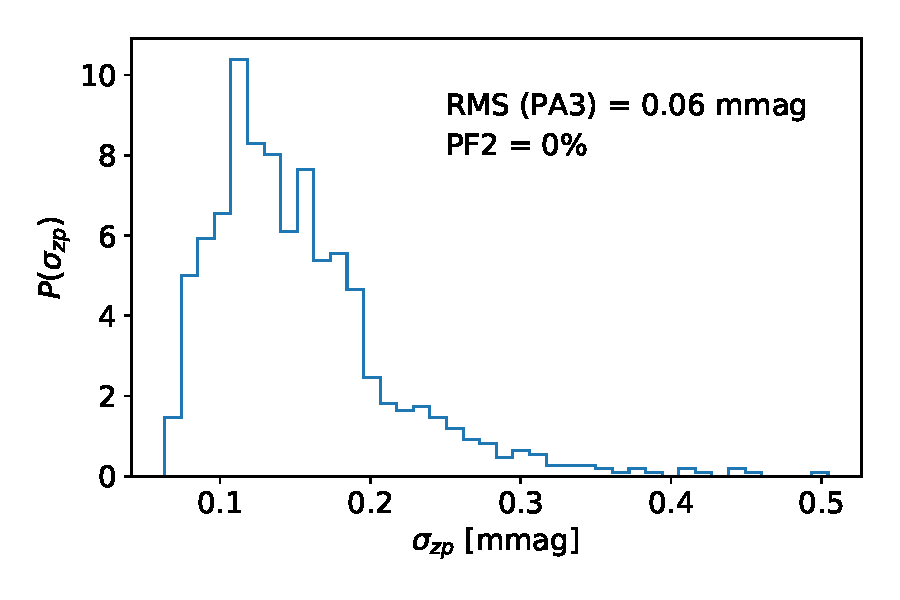
\includegraphics[width=0.85\columnwidth]{PA234.pdf}
\caption{Normalized distribution of the error in the zeropoint value, $\sigma_{zp}$ for 1000 randomly selected sensor-visits. We see that the distribution is quite asymmetrical and find that the RMS (PA3) is 0.06 mmag, fulfilling the requirements in the LSST-SRD (15 mmag). We also find that only 0\% (PF2) of the visits deviate from the median more than 20 mmag, in compliance with the LSST-SRD requirements.}
\label{fig:PA34}
\end{figure}

These tests show that the processing pipeline behaves as expected but also, that our images are generated with consistent zeropoints.

\subsubsection{Depth requirements}
\label{sssec:depth}
In order to observe the object number density required to fulfill the science goals of LSST and DESC, the LSST-SRD sets some requirements in the minimum per-visit image depth for images with fiducial sky brightness of 21 mag/arcsec$^2$, exposure time of 30 s, airmass=1 and fiducial seeing (FWHM) of 0.7 arcseconds. In order to mimic this we select the visits that fulfill the following criteria~\citep{LPM-17}:
\begin{itemize}
\item Altitude $> 80$ degrees.
\item $0.68\arcsec <$ seeing (FWHM) $ < 0.71\arcsec$
\item Sky-brightness (in $r$-band) $ \geq 21$ 
\end{itemize}
We obtain a total of 520 sensor-visits fulfilling these criteria. We then compute the median 5-$\sigma$ depth  using the magnitude errors (as described later in the text) and compare with the predicted depth by OpSim. After this, we check that the median of the depth distribution is larger than the minimum depth (D1=DB1=24.3 mag) as defined in the LSST-SRD. In order to have a uniform, well characterized sample, depth uniformity is already required. This is why we also check that no more than 20\% of the visits have a depth lower than Z1=24.0 by computing the lower 20th percentile in the depth distribution. The results of these checks are depicted in \figref{DF1_checks}. We find that the median of the depth distribution in the selected visits, $24.297 \pm 0.009$ mag, is compatible (within a standard deviation of the mean) with the minimum depth set in the LSST-SRD. We find as well that the 20th percentile, Z1=24.1, is larger than the minimum value set in the LSST-SRD. We also check that in a given visit, the variation in the field-of-view is within the requirements. The LSST-SRD establishes that, in a representative visit with depth D1 no more than 20\% of the field-of-view will be (Z2) 0.4 magnitudes brighter than the nominal (24.3). We select visit 2218486 since its median depth is 24.3. We find that the 20th percentile is 24.29 fulfilling the criteria. This test demonstrates that we generate images with the required depth and in concordance with our inputs.

\begin{figure}
\centering
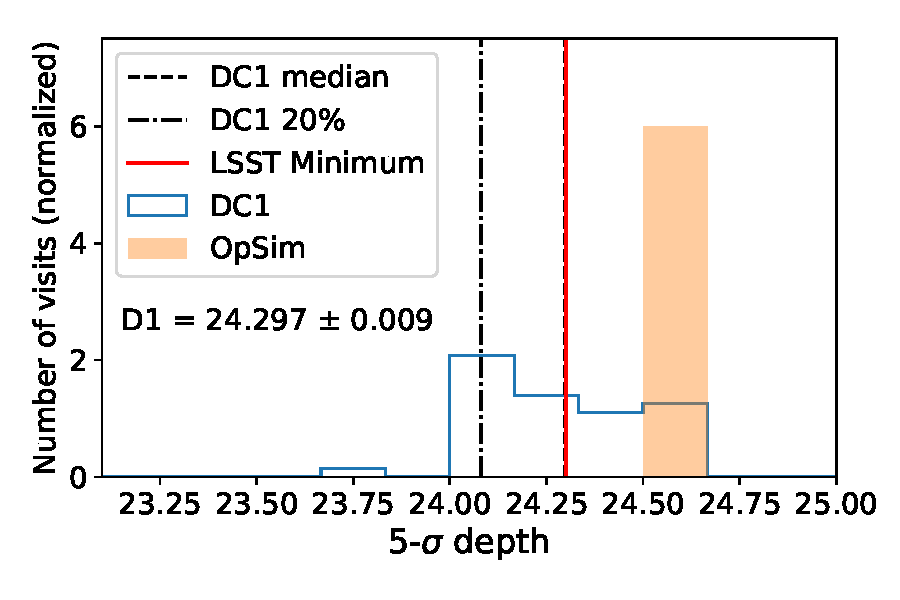
\includegraphics[width=0.85\columnwidth]{m5_goals}
\caption{Measured depth in visits with Altitude $>80$ deg., $0.68 \arcsec <$ seeing $ < 0.71 \arcsec$ and Sky-brightness (in $r$-band) $\geq 21$ (blue histogram) compared to the predicted depth by OpSim (solid orange histogram). The median of this distribution (dashed line) is very close to the LSST-SRD minimum depth D1=24.3 (red vertical line), the 20th percentile is also shown and we can appreciate that is larger than Z1=24.0 as established by the LSST-SRD.}
\label{fig:DF1_checks}
\end{figure}

\subsubsection{PSF requirements}
\label{sssec:psf}
The LSST-SRD sets criteria regarding the maximum modulus of the PSF ellipticity, $|e|$, mostly driven by weak lensing analyses. We use the distortion definition for $|e|$~\citep{1991ApJ...380....1M}:
\begin{equation}
|e| = \frac{a^{2} - b^{2}}{a^{2}+b^{2}},
\end{equation}
where $a, b$ are the semi-major and semi-minor axes of the PSF. We test exposures with PSF-FWHM $\approx 0.69\arcsec$ and no more than 10 degrees away from zenith and check that the median ellipticity is no larger than 0.05 (SE1) and that no more than 10\% of the images exceed 0.1 (SE2). Our analytic (and circularly-symmetric) PSF models should, by design, fulfill these criteria. However, we have to test if the reconstructed PSF also fulfills them. The PSF was reconstructed using the PSFEx~\citep{2011ASPC..442..435B} implementation in the LSST software stack. We tested this in the processed data by using the same 520 sensor-visits used to check the depth requirements described above. We checked the modulus of the PSF ellipticity at the position of the detected objects in these visits accumulating them in the histogram shown in \figref{SE1_DC1}. We obtained that SE1=0.001 and SE2=0.002, below the maximum values allowed by the LSST-SRD. In future data challenges, we will use more realistic PSF models and we expect these margins to be different.
\begin{figure}
\centering
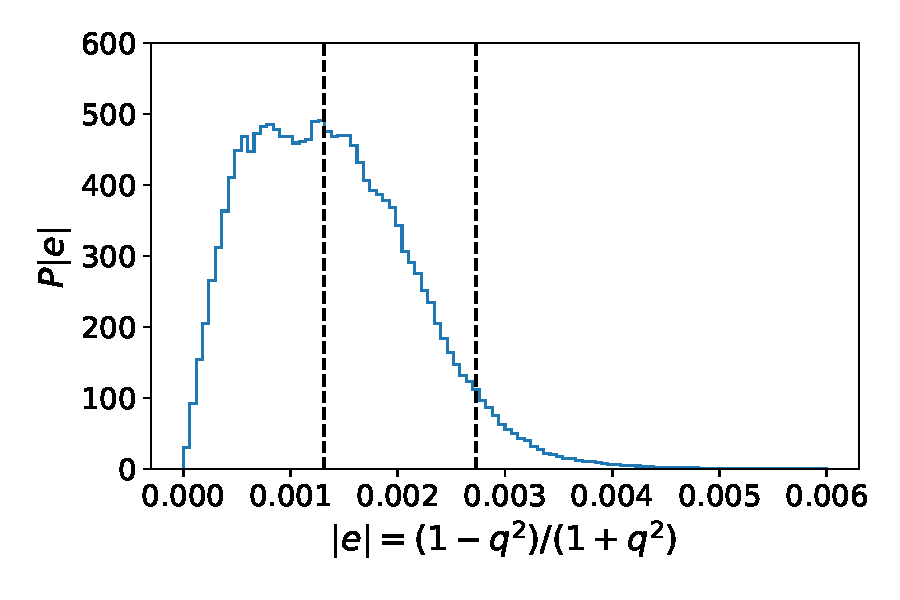
\includegraphics[width=0.85\columnwidth]{PSF_ellipticity_DC1}
\caption{PSF ellipticity distribution accumulated for 520 sensor-visits measured at the position of detected objects. The median (SE1=0.001) and 90th (SE2=0.002) percentiles are shown as the dashed lines. Note that these values are an order of magnitude lower than the specifications by the LSST-SRD (SE1=0.05 and SE2=0.1, respectively).}
\label{fig:SE1_DC1}
\end{figure}

We also check that, in these images, 85\% of the point-like sources flux is contained within $0.80\arcsec$ or less (SR1), 95\% within $1.31\arcsec$ or less (SR2) and 99\% within $1.81\arcsec$ (SR3) or less. In our case we obtain SR1$=0.64\arcsec$, SR2$=1.01\arcsec$ and SR3$=1.79\arcsec$. This was done by calculating the radius at which the PSF was at its 85th, 95th and 99th percentiles.

For weak lensing analyses, correct modeling of the PSF is crucial~\citep{2004MNRAS.353..529H} and both the LSST-SRD and the DESC-SRD contain explicit requirements about PSF residuals. In particular, the LSST-SRD states that using the full survey data the auto- and cross-correlations ($E_{1}, E_{2}, E_{X}$) of the PSF residuals over an arbitrary field-of-view should be below TE1 (3 $\times 10^{-5}$) for $\theta \leq 1$ arcmin, below TE2 ($3 \times 10^{-7}$) for $\theta \geq 5$ arcmin and no more than 15\% of the images will have median larger than TE3 ($6 \times 10^{-5}$) for $\theta \leq 1$ arcmin and, TE4 ($5 \times 10^{-7}$) for $\theta \geq 5$ arcmin. 

To check these criteria we calculate $E_{1}, E_{2}, E_{X}$ using the definitions of the LSST-SRD:
\begin{eqnarray}
e_{1} = \frac{\sigma^{2}_{1} - \sigma^{2}_{2}}{\sigma_{1}^{2}+\sigma_{2}^{2}},\\
e_{2} = \frac{2\sigma^{2}_{12}}{\sigma_{1}^{2}+\sigma_{2}^{2}},\\
E_{1} (\theta) = \langle \delta e^{(i)}_{1}\delta e^{(j)}_{1} \rangle,\\
E_{2} (\theta) = \langle \delta e^{(i)}_{2}\delta e^{(j)}_{2} \rangle,\\
E_{X} (\theta) = \langle \delta e^{(i)}_{1}\delta e^{(j)}_{2} \rangle.
\end{eqnarray}
The quantities $\sigma_{1}^{2}, \sigma_{2}^{2}$ are the second order moments of a source along some set of perpendicular axes and $\sigma^{2}_{12}$ is the covariance, $\delta e_{1}, \delta e_{2}$ are the residuals, and the angular brackets indicate averaging over all pairs of stars $i$, $j$ at a given angular separation $\theta$.

In practice, we compute the PSF-corrected moments of high signal-to-noise (SNR $>$ 100) stars across the field of view using \texttt{TreeCorr}~\citep{2004MNRAS.352..338J}. Our findings are shown in \figref{TEx}. We can see that for $E_{1}$, $E_{2}$, and $E_{X}$ the TE1 criterion is fulfilled as well as TE2. We ignore TE3 and TE4 because we expect our images to fulfill these criteria automatically, given that we use the same analytic form for the PSF for all visits. 

\begin{figure}
\centering
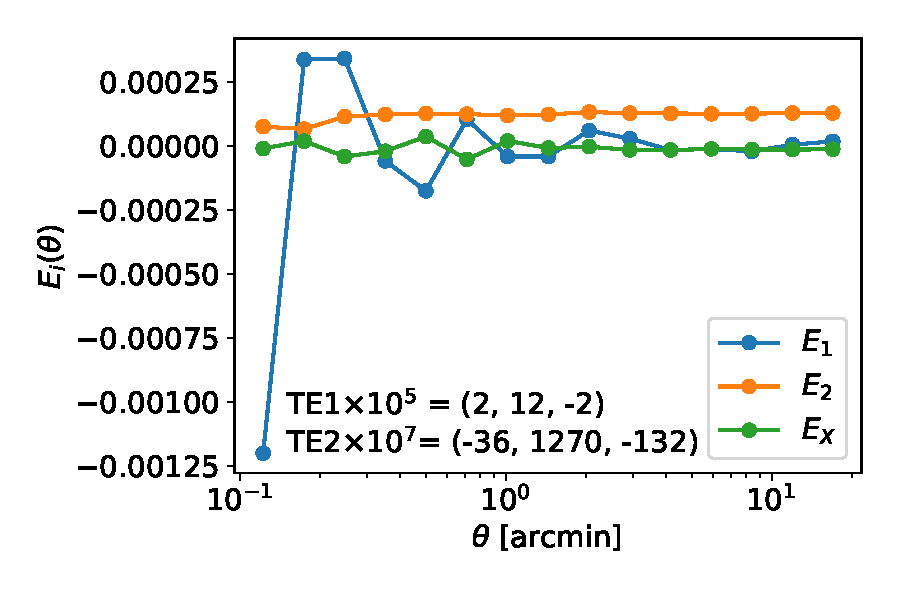
\includegraphics[width=0.85\columnwidth]{TEx}
\caption{Auto and cross-correlation functions, $E_{1}$ (blue), $E_{2}$ (orange), $E_{X}$ (green) of the PSF residuals as a function of the aperture angle $\theta$. We see that our data fulfill the LSST-SRD requirements.}
\label{fig:TEx}
\end{figure}

Finally, the DESC-SRD requires (WL4-Y10) that the systematic uncertainty in the PSF model defined using the trace of the second moment matrix should not exceed 0.1\% for full-depth (Y10) DESC weak lensing analysis. We randomly select 3000 visits, obtain the input and measured PSF, and measure the trace of the second order moments, $T$ with GalSim. We then compute the relative difference, $\Delta T/T$, obtaining the results depicted in \figref{WL4-Y10}. We find that our dataset shows that the standard deviation of the distribution is 0.05\%, lower than the requirement.
\begin{figure}
\centering
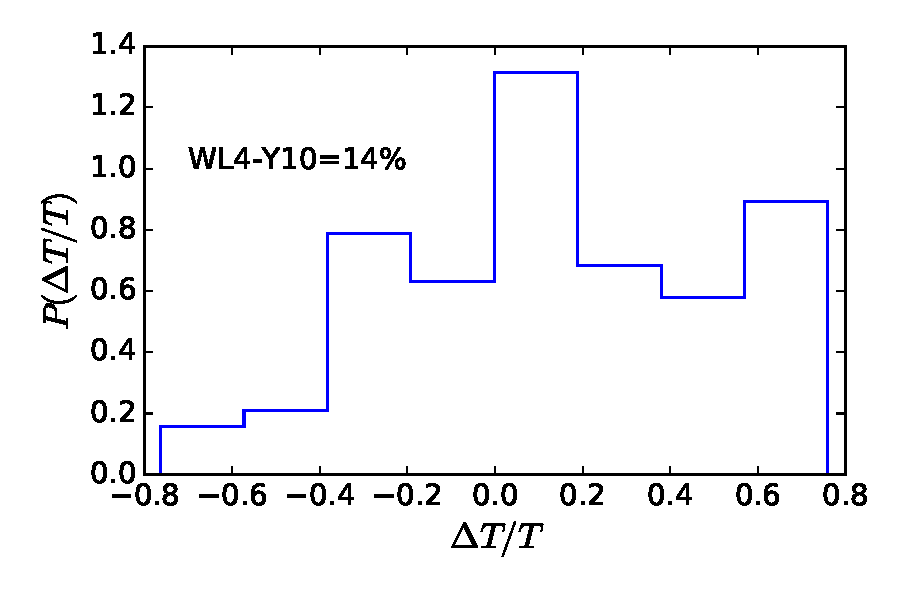
\includegraphics[width=0.85\columnwidth]{WL4-Y10}
\caption{Normalized distribution of the relative difference in the trace of the second order moments, $\Delta T/T$ between input and output PSF. We see that the standard deviation of the distribution (WL4-Y10) is 0.05\%, much complying with the requirement (0.1\%).}
\label{fig:WL4-Y10}
\end{figure}

As seen in Table~\ref{tab:kpm_table}, our images and catalogs pass all the requirements by a good margin, demonstrating our ability to both generate and process high-quality data. We can also see that some of the criteria (e. g., number of filters used) do not pass the requirements due to design choices and do not affect the science analyses that can be performed with this dataset.

%\begin{table}[h!]
%\centering
%\begin{tabular}{|c|c|c|c|}
%\hline
%Quantity (LSST-SRD) & Minimum & DC1 & Passed\\
%\hline
%Filter complement & ugrizy & r & \textcolor{blue}{N}\\
%Nfilters & 3 & 1 & \textcolor{blue}{N}\\
%Nv1 & 184 & 184 & \textcolor{blue}{Y}\\
%pixSize (arcsec) & 0.22 & 0.2 & \textcolor{blue}{Y}\\
%AA1 (milliarcsec) & 100 & 20 & Y\\
%PA1 (millimag) & 8 & 6 & Y\\
%PF1 (\%) & 20 & 17 & Y\\
%PA2 (millimag) & 15 & - & -\\
%PA3 (millimag) & 15 & 0.06  & Y\\
%PF2 (\%) & 20 & 0 & Y\\
%PA4 (millimag) & 20 & - & -\\
%%PA5 (millimag) & 10 & 1.4 & check\\
%PA6 (millimag) & 20 & 17 & Y\\
%AM1 (milliarcsec) & 20 & 8 & Y\\
%AF1 (\%) & 20 & 13 & Y\\
%AD1 (milliarcsec) & 40 & - & -\\
%AM2 (milliarcsec) & 20 & 4 & Y\\
%AF2 (\%) & 20 & 9 & Y\\
%AD2 (milliarcsec) & 40 & - & -\\
%AM3 (milliarcsec) & 30 & 7 & Y\\
%AF3 (\%) & 20 & 2 & Y\\
%AD3 (milliarcsec) & 50 & - & -\\
%%Fleak (\%) & 0.02 & 0 & \textcolor{blue}{Y}\\
%%FleakTot (\%) & 0.1 & 0 & \textcolor{blue}{Y}\\
%D1 (mag) & 24.3 & 24.3 & Y\\
%DF1 (\%) & 20 & - & -\\
%Z1 (mag) & 24.0 & 24.1 & Y\\
%DB1 (mag/r-band) & 24.3 & 24.3 & Y\\
%DF2 (\%) & 20 & - & -\\
%Z2 (mag) & 0.4 & 0.1 & Y\\
%%S1 (0.44) & 0.59 & check & check\\
%%S1 (0.60) & 0.72 & check & check\\
%%S1 (0.80) & 0.89 & check & check\\
%%SF1 (\%) & 10 & check & check\\
%%SX & 1.2 & check & check\\
%%SXE & 0.59 & check & check\\
%SE1 & 0.04 & 0.001 & Y\\
%EF1 & 10 & - & -\\
%SE2 & 0.1 & 0.002 & Y\\
%SR1 (arcsec) & 0.80 & 0.64 & Y\\
%SR2 (arcsec) & 1.31 & 1.01 & Y\\
%SR3 (arcsec) & 1.81 & 1.79 & Y\\
%TE1 & $3 \times 10^{-5}$ & $3\times 10^{-6}$ & Y\\
%TE2 & $3 \times 10^{-7}$ & $9\times 10^{-8}$ & Y\\
%%TEF & 15\% & - & -\\
%%TE3 & $6 \times 10^{-5}$ & - & N\\
%%TE4 & $5 \times 10^{-7}$ & - & N\\
%\hline
%\end{tabular}
%\caption{Table with the Key Performance Metrics (KPMs) that we used to check the quality of our end-to-end pipeline. The criteria that are passed or not due to design choices are shown in blue. We mark with dashes the quantities that we use as auxiliary to compute some of the criteria, e.g., we use EF1 to compute SE2.}
%\label{tab:kpm_table}
%\end{table}
%
%\begin{table}[h!]
%\centering
%\begin{tabular}{|c|c|c|c|}
%\hline
%Quantity (DESC-SRD) & Maximum & DC1 & Passed \\
%\hline
%WL4-Y10 (\%) & 0.1 & 0.05 & Y\\
%%WL5-Y10 (\%) & 0.1 & N/A & N/A\\
%\hline
%\end{tabular}
%\caption{Criteria from the DESC-SRD tested in the DC1 simulation. This document also includes other criteria that cannot be tested with our data but will be relevant for future data challenges.}
%\label{tab:desc_srd_table}
%\end{table}

\section{Data selection and masking}
\label{sec:data_selection}
In this section, we describe how we take advantage of the fact that we have full knowledge about the simulated sources in order to get a ``clean" data sample for clustering tests, we also describe the catalog mask and how we generate maps of different observational effects (seeing, sky-brightness, etc.) present in the simulation. Unless explicitly stated, the procedures and selections made in this section are performed in both the dithered and undithered simulations.

\subsection{Sample selection}
\label{ssec:sample_selection}

In this subsection we are going to use the spatial+magnitude technique to identify flags or thresholds in variables that may allow us to get a clean sample for clustering. In principle, given that the LSST DM software stack is essentially the same as the HSC reduction pipeline used in~\citet{2018PASJ...70S..25M}, we could potentially perform similar cuts. However, note that we are working in $r$-band only, so some of the required cuts cannot be performed. In addition, some variables, such as the so-called blendedness parameter, used in~\citet{2018PASJ...70S..25M}, are not available in the version of the LSST DM software stack that we ran to process the data (\texttt{v13.0}). As a consequence, we propose our own selection cuts, although we follow the criteria in~\citet{2018PASJ...70S..25M} as guidance.


The methodology to perform the selections is simple: we check the primary detected sources that have no match using the spatial+magnitude technique and we compute the fraction of objects that are flagged, $f_{u,i} = N_{flag_{i}, unmatched}/N_{total, unmatched}$, and compare it to the corresponding fraction of flagged matched primary detected sources, $f_{m,i} = N_{flag_{i}, matched}/N_{total, matched}$, for each one of the flags, $flag_{i}$, in the catalog. If the ratio $f_{u,i}/f_{m,i}$ is larger than 50 for a particular flag and $f_{m,i} < 0.01$, i.e., less than 1\% of the matched primary sources have that flag, it means that the presence of that flag is a good indicator of problematic sources. Thus, we eliminate the sources with those flags. We also repeat the same procedure looking for the absence of a certain flag or whether a quantity is frequently measured as not a number, \texttt{NaN}, and check for redundant cuts. 


%The results of the selection process are shown in \figref{flags_DC1}. In this Figure we can see that most of the flags shown have a larger impact in measured sources that have no match in the input catalog (unmatched). 

We notice that some of the flags are very efficient distinguishing unmatched from matched objects. For example, \texttt{base\_ClassificationExtendedness\_flag = True}, which means that there was a failure at the time of deciding whether a source was extended or point-like, eliminates more than 30\% of the objects with no match, while barely affecting the matched objects. There are other three flags pretty efficient to filter out unmatched objects but, in case of using them, we would lose $\approx 50\%$ of our sample. These include \texttt{modelfit\_CModel\_flags\_smallShape==False} which means that the initial parameter guess did not result in a negative radius (if \texttt{True} the initial guess for the radius would be negative). Intuitively, we expect this flag to be \texttt{False} for well-behaved objects and thus, we should not use this for our selection. Another case where the ratio of flagged unmatched (and matched) objects is very large is \texttt{modelfit\_CModel\_flags\_region\_usedFootprintArea==True}, which means that the pixel region for the initial fit was defined by the area of the footprint. This flag, again, is not necessarily indicative of problems with the measured object. Finally, we see that \texttt{modelfit\_CModel\_flags\_region\_usedPsfArea==False} also affects a very large fraction of unmatched and matched objects. These objects are such that the pixel region for the initial fit was not set to a fixed factor of the PSF area, which is not indicative of any problems with the source. A summary of the effects of these cuts can be found in Table~\ref{tab:summary_flag_selection}.

%\begin{figure*}
%\centering
%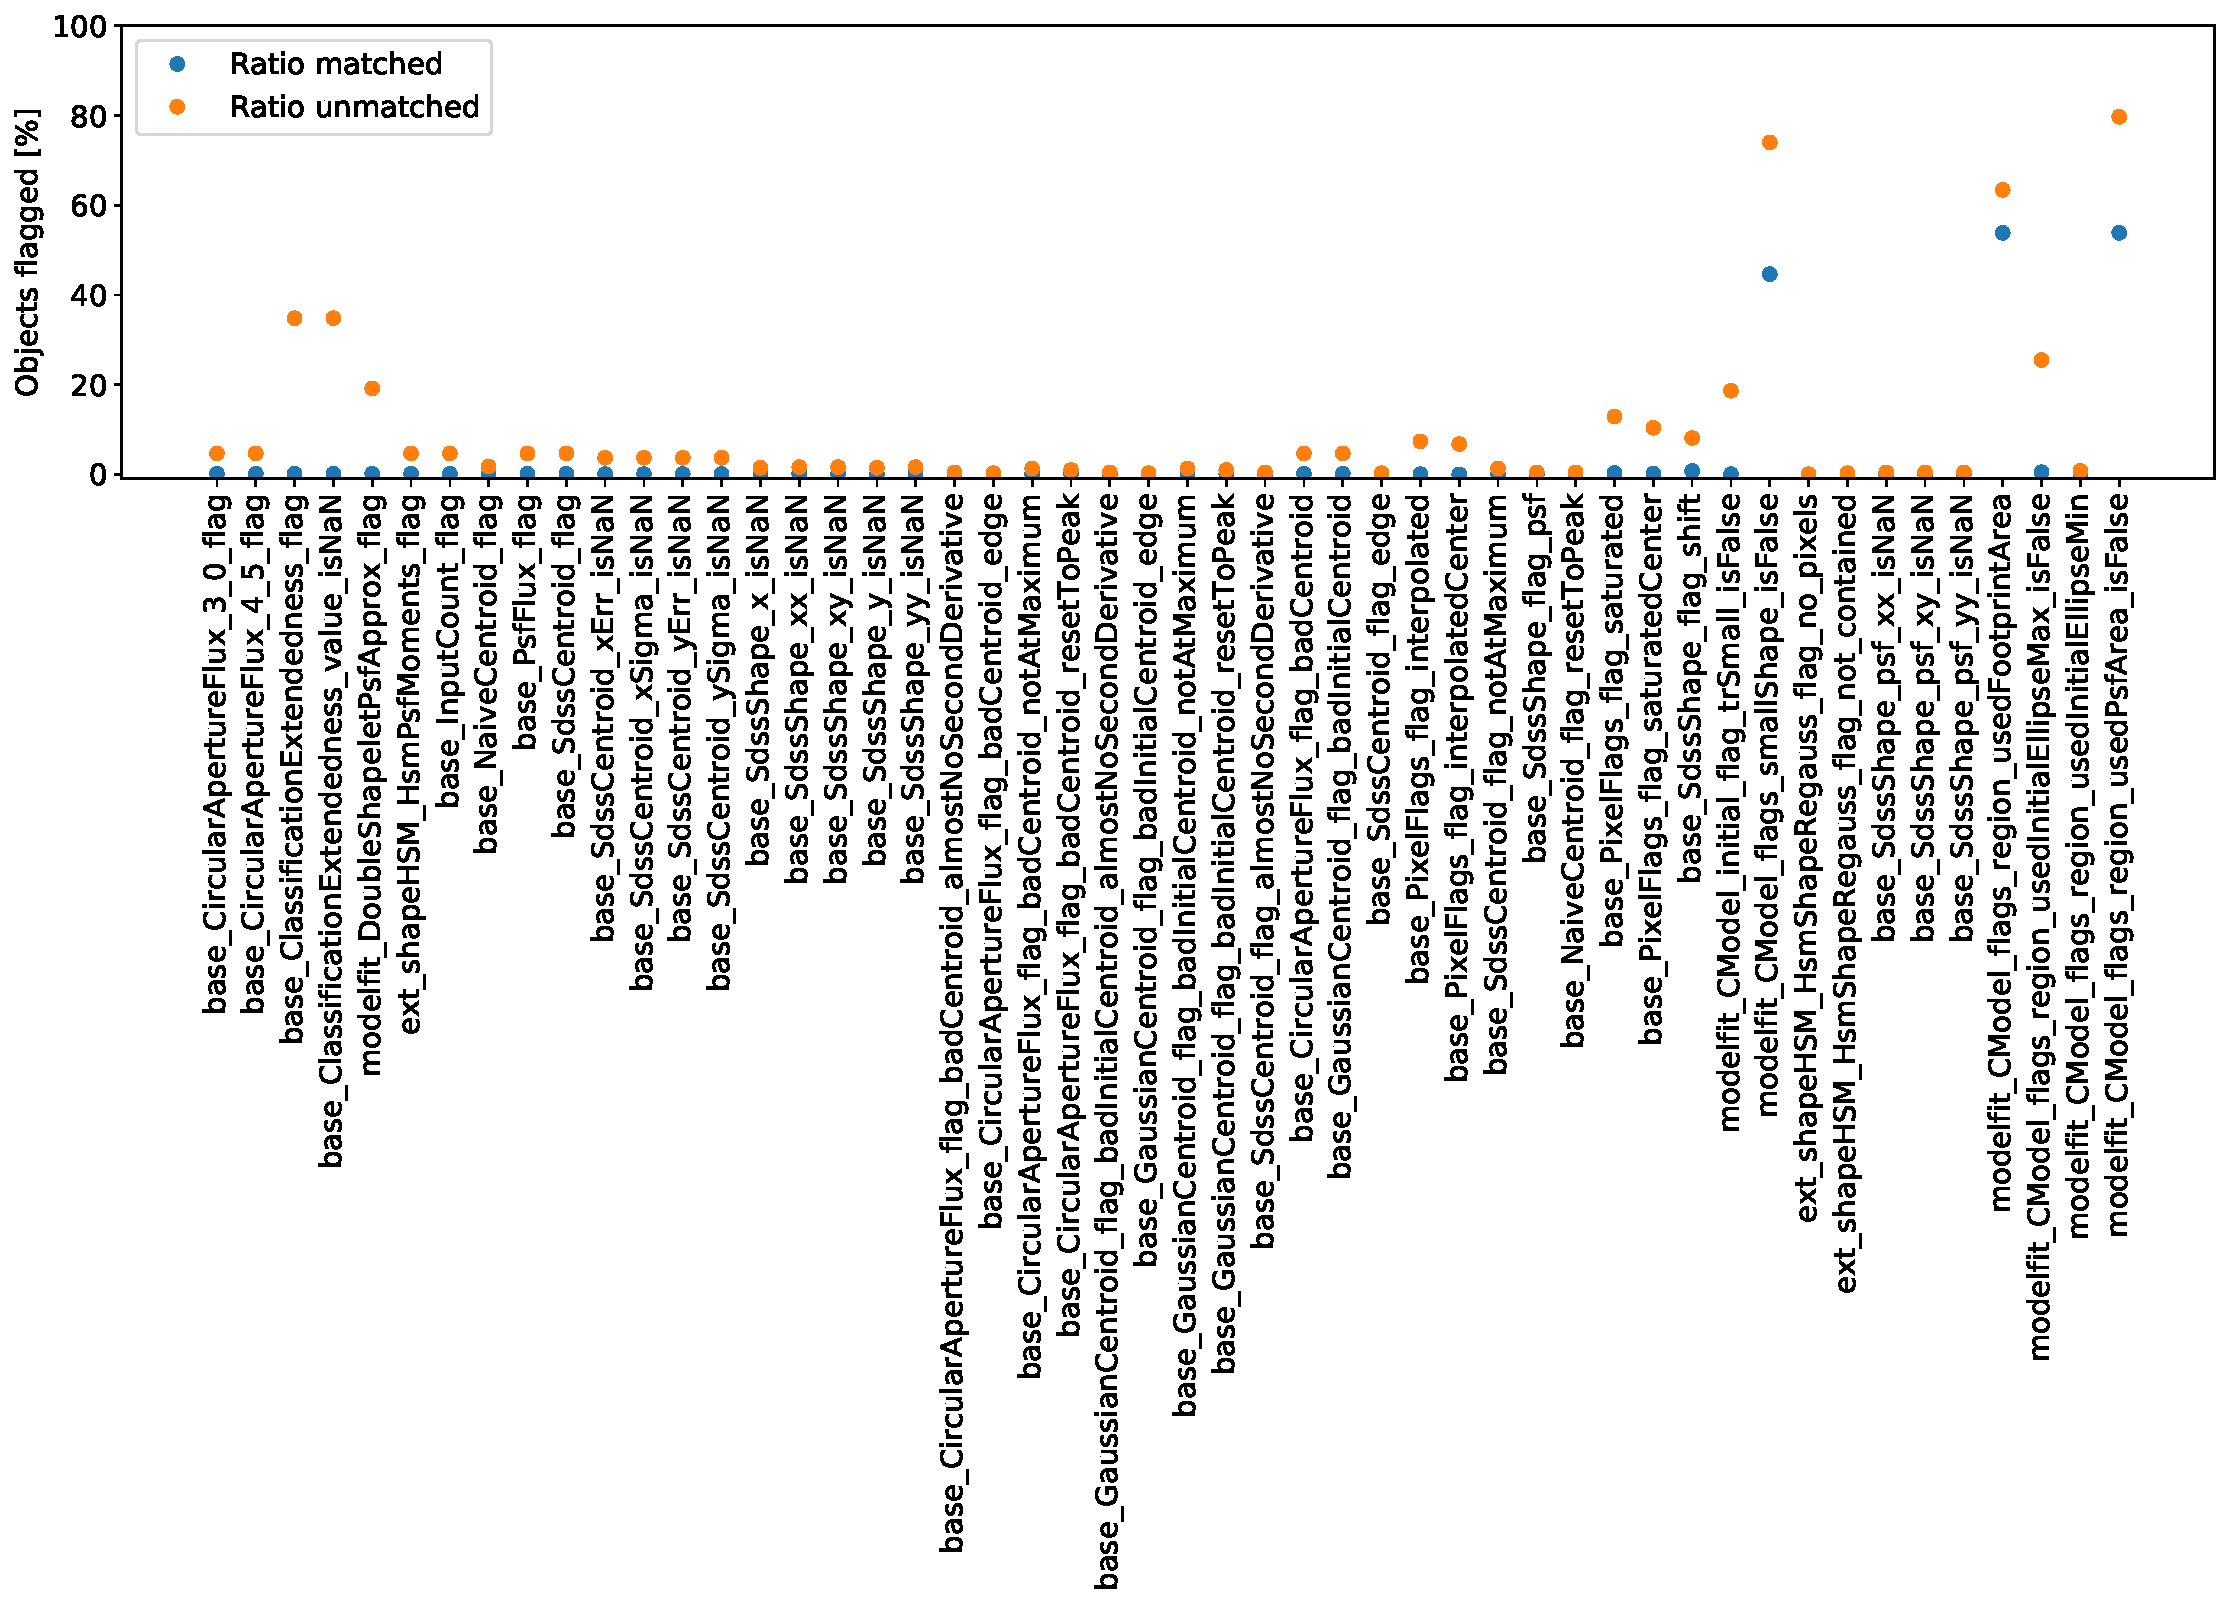
\includegraphics[width=0.9\textwidth]{flags_DC1}
%\caption{Percentage of flagged objects with a match in the (solid blue circles) and flagged objects with no match in the truth catalog (orange solid circles) as a function of each flag. We show only flags where there is either a large fraction of objects with no match compared to objects with a match or where more than 50\% of the objects have been flagged and the fraction of unmatched objects is larger than the ratio of matched objects.}
%\label{fig:flags_DC1}
%\end{figure*}

As a result, \textbf{we eliminate} from our selection all the sources that fulfill at least one of the following conditions:
\begin{itemize}
\item \texttt{detect\_isPrimary = False}. As discussed earlier, this means that the source has not been fully deblended or is outside of the inner region in a coadd.
\item \texttt{base\_NaiveCentroid\_flag = True}. This means that there is a general failure during the source measurement.
\item \texttt{base\_SdssShape\_flag\_psf = True}. This means that there is a failure in measuring the PSF model shape in that position.
\item \texttt{ext\_shapeHSM\_HsmSourceMoments\_flag\_not\_contained = True}. This means that the center of the source is not contained in its footprint bounding box.
\item \texttt{modelfit\_DoubleShapeletPsfApprox\_flag = True}. This means that there is a general failure while performing the double-shapelet approximation to the PSF model in the position of this source (see Appendix 2 in~\citet{2018PASJ...70S...5B} for more details).
\item \texttt{base\_PixelFlags\_flag\_interpolated = True}. This means that there are interpolated pixels in the source's footprint.
\item \texttt{base\_PixelFlags\_flag\_interpolatedCenter = True}. This means that the center of a source is interpolated.
\item \texttt{base\_PixelFlags\_flag\_saturatedCenter = True}. This means that the center of a source is saturated.
\item \texttt{base\_ClassificationExtendedness\_flag = True}. This means that there is a general failure when using the extendedness classifier.
\item \texttt{modelfit\_CModel\_flags\_region\_usedInitialEllipseMin = True}. This means that the pixel region for the final model fit is set to the minimum bound used in the initial fit.
\item \texttt{base\_SdssShape\_x/y = NaN}. This means that the centroid position (either in the x or y axes) is measured as NaN.
\item \texttt{base\_SdssCentroid\_x/yErr = NaN}. This means that the error in the centroid position (either in the x or y axis) is measured as NaN.
\end{itemize}

After these cuts we keep 8.25 million objects in the dithered catalog and 7.51 million objects in the undithered catalog. We will refer to this sample as the \textit{clean sample}. After the cuts, the ratio of unmatched objects decreases by $\approx 60\%$ from $\sim 5\%$ (of the catalog before cuts) to $\sim 3\%$ (of the clean sample), while we retain $99.7\%$ of the matched objects. In DC1 we are limited by only having $r$-band information. The addition of other imaging bands will provide additional independent information that will decrease the fraction of noise fluctuations that make it into the catalog and that can allow to further clean the sample (e.g., by performing selection cuts in color-color diagrams).

\begin{table}
\centering
\begin{tabular}{|c|c|c|}
\hline
Cuts & Matched $[\%]$ & Matched kept $[\%]$\\
\hline
Primary detected & 95.2 & 100\\
Clean sample & 96.5 & 99.7\\
%All flags in \figref{flags_DC1} & 98.7 & 32.3\\ 
\hline
\end{tabular}
\caption{Summary of selection efficiency and purity for the different flag cuts that we explore in DC1.}%\figref{flags_DC1}.}
\label{tab:summary_flag_selection}
\end{table}

We now focus on how many of these objects are matched as a function of magnitude and signal-to-noise ratio. In \figref{snr_mag_selection}, we can see that the fraction of unmatched objects grows very quickly for $r > 26$, and for SNR$<6$. Therefore, $r < 26$ and/or SNR$>6$ look like sensible selection criteria to ensure good quality data. In particular, we select our \textit{final sample} using the following criteria:

\begin{itemize}
\item \texttt{base\_ClassificationExtendedness\_value=1}.
\item $20 \leq$ \texttt{r\_mag\_CModel} $\leq 25.5$. 
\end{itemize}

These selection cuts ensure a low fraction of unmatched objects and also, as we will justify in following sections, good purity of our galaxy sample (low stellar contamination).

\begin{figure}
\centering
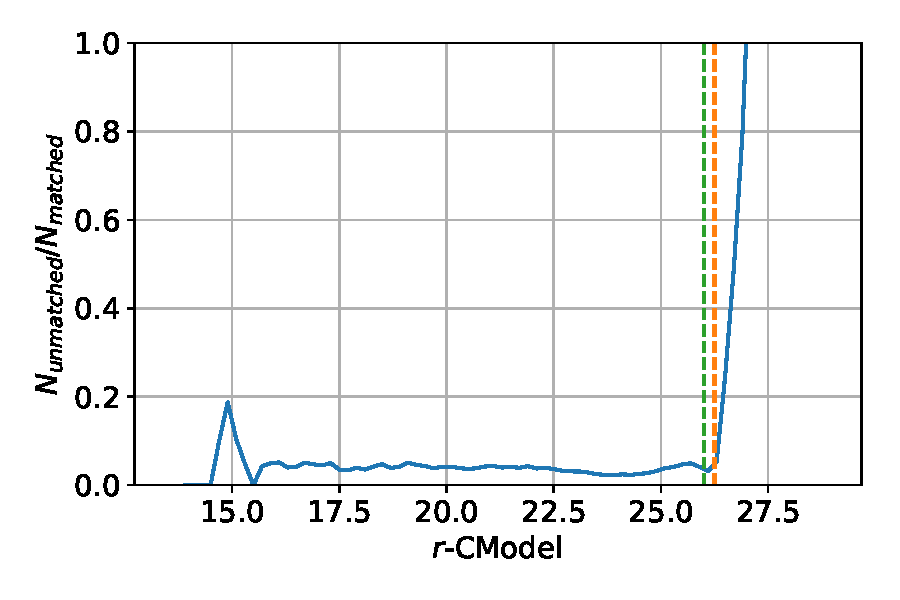
\includegraphics[width=0.9\columnwidth]{unmatched_fraction_magnitude.pdf}
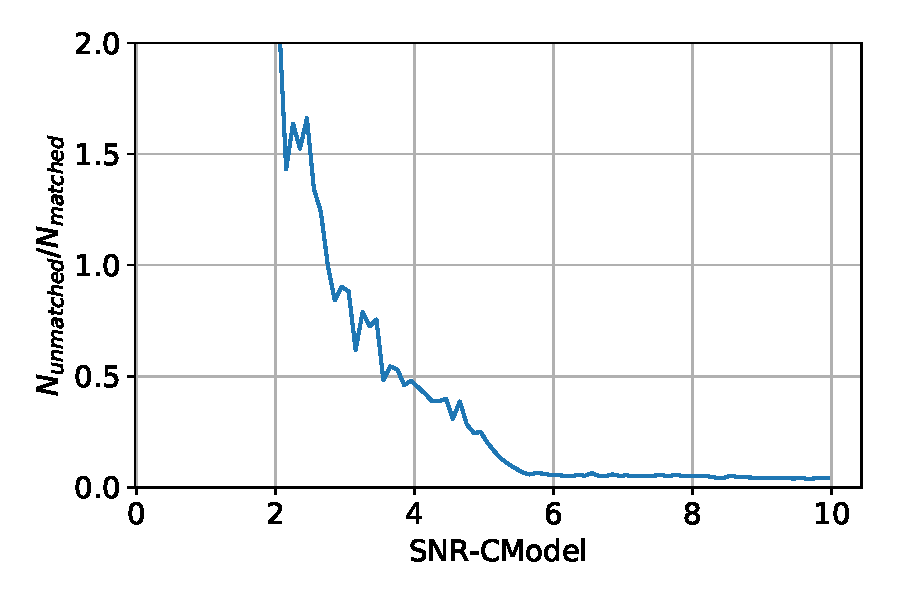
\includegraphics[width=0.9\columnwidth]{unmatched_fraction_SNR.pdf}
\caption{Top: Ratio of unmatched to matched primary detected sources after selection cuts as a function of magnitude. The dashed vertical lines show the median depth for the dithered (orange) and undithered (green) fields. Bottom: Ratio of unmatched to matched primary detected sources after selection cuts as a function of SNR.}
\label{fig:snr_mag_selection}
\end{figure}

\subsection{Star/galaxy classification}

For weak lensing and clustering analyses, it is important to have a pure galaxy sample and a good control over the fraction of stars that are classified as galaxies. Our pipeline includes the variable \texttt{base\_ClassificationExtendedness\_value} (see~\citet{2018PASJ...70S...5B} for more details) , which we will refer to as extendedness, and can be used as a proxy to separate stars from galaxies as shown in~\citet{2018PASJ...70S..25M} and~\citet{2018PASJ...70S...5B}. In this work we say that an object has been classified as a galaxy if extendedness=1, and that the object has been classified as a star if extendedness=0. To evaluate extendedness as star/galaxy classifier in DC1, we use the \textit{final sample} (avoiding the extendedness cut) in the dithered field, although we find similar results using the undithered field, and match it to our input catalog using the S+M method. After that, we follow~\citep{2018MNRAS.481.5451S} and compute the true positive rate (TPR), usually referred to as \textit{completeness}, and positive predictive value (PPV), usually called \textit{purity}, defined as:
\begin{eqnarray}
\mathrm{TPR} = \frac{\mathrm{True Positive}}{\mathrm{True Positive}+\mathrm{False Negative}}, \\
\mathrm{PPV} = \frac{\mathrm{True Positive}}{\mathrm{True Positive}+\mathrm{False Positive}}.
\end{eqnarray}
For galaxies, true positive are objects classified as galaxies and matched to galaxies; false negative are objects classified as stars but matched to galaxies; and false positive are objects classified as galaxies but matched to stars. This way, we know the total stellar (or galaxy) contamination as a function of measured magnitude. The results are depicted in \figref{star_galaxy_separation}. We see that at the fainter end ($r \approx 26$), the PPV (purity) of the galaxy sample (and of the stellar sample) using the extendedness classifier starts to decrease, getting as low as 95\% for the last bin in our analysis, and an overall $f_{star}=1.4\%$. For a more restricted magnitude threshold of $r < 25$ we can get $f_{star} = 0.7\%$. Note that these numbers are larger than those presented in~\citet{2018PASJ...70S..25M}. This is mostly due to the fact that our PSF is larger, making the extendedness classifier perform a little bit worse, and that we do not include any cuts in resolution. However, this level of stellar contamination is acceptable for the purposes in this work. Note that this selection is optimized for galaxy purity and completeness and should be modified for stellar studies.

\begin{figure}
\centering
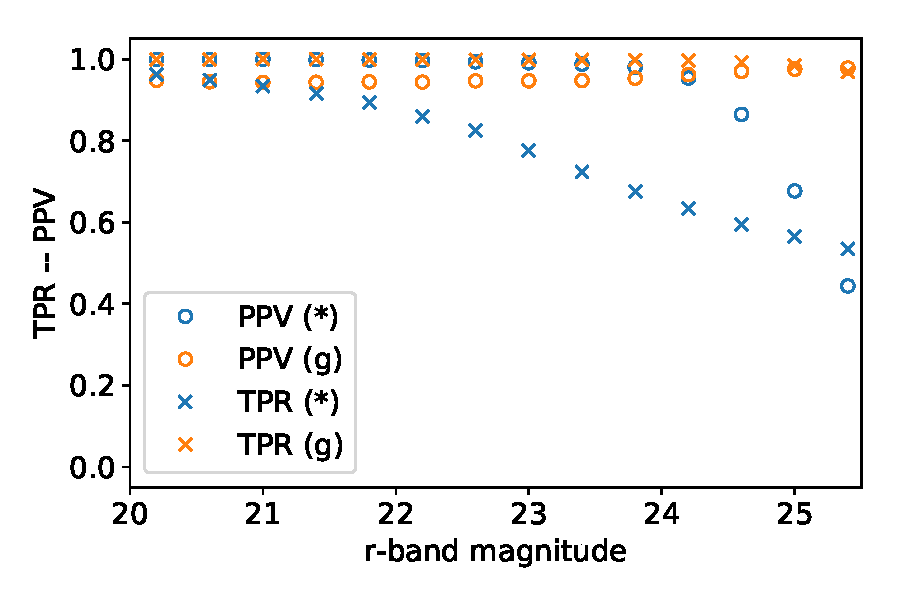
\includegraphics[width=0.9\columnwidth]{stellar_contamination_v2}
\caption{Performance of the \texttt{base\_ClassificationExtendedness\_value} as star-galaxy classifier as a function of magnitude. This classifier has been optimized for galaxy purity and completeness. We show the true positive rate (TPR) for stars (dark crosses) and galaxies (light crosses) and the positive predictive value (PPV) for stars (dark open circles) and galaxies (light open circles). Both the TPR and PPV for galaxies is high in the range of magnitudes that we are studying.}
\label{fig:star_galaxy_separation}
\end{figure}
\subsection{Depth maps and footprint masking}
\label{sec:masking}

In order to estimate the depth in the coadd catalogs we generate a flat-sky map, with resolution of $1.74$ arcminutes, containing the detected primary sources in the \textit{clean sample} from the previous subsection. This resolution allows us to accurately estimate the power-spectra up to $\ell \sim 6000$, where the power-spectra will be mostly dominated by shot-noise. Then, for each cell in the map, we bin the objects in magnitude and compute which magnitude bin corresponds to SNR=5.

These maps are shown in \figref{depth_maps}. We can see that the dithered simulation is indeed very uniform ($> 50\%$ of its footprint lie in the same depth bin) showing the success of the dither strategy. However, we can see that in the undithered simulation, as expected, there are zones with a higher depth (the overlap of the pointing positions) and a reduced median depth.
\begin{figure}
\centering
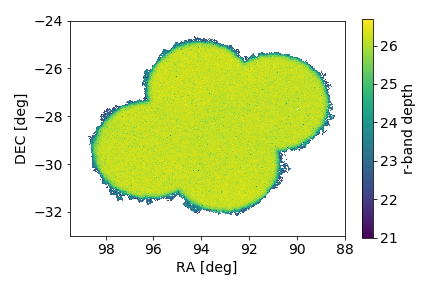
\includegraphics[width=0.85\columnwidth]{dithered_depth.png}
%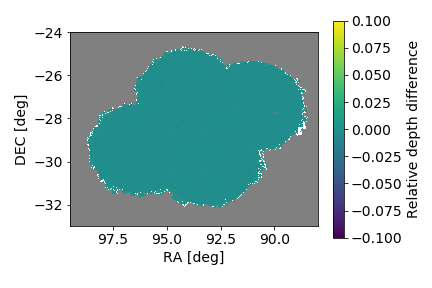
\includegraphics[width=0.45\textwidth]{dithered_difference.png}
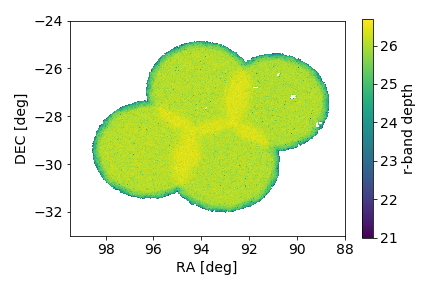
\includegraphics[width=0.85\columnwidth]{undithered_depth.png}
%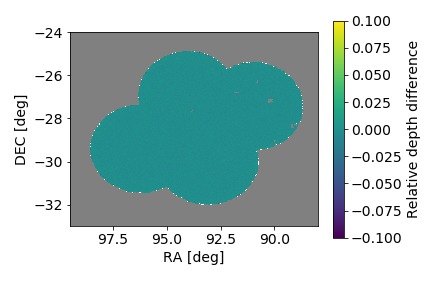
\includegraphics[width=0.45\textwidth]{undithered_difference.png}
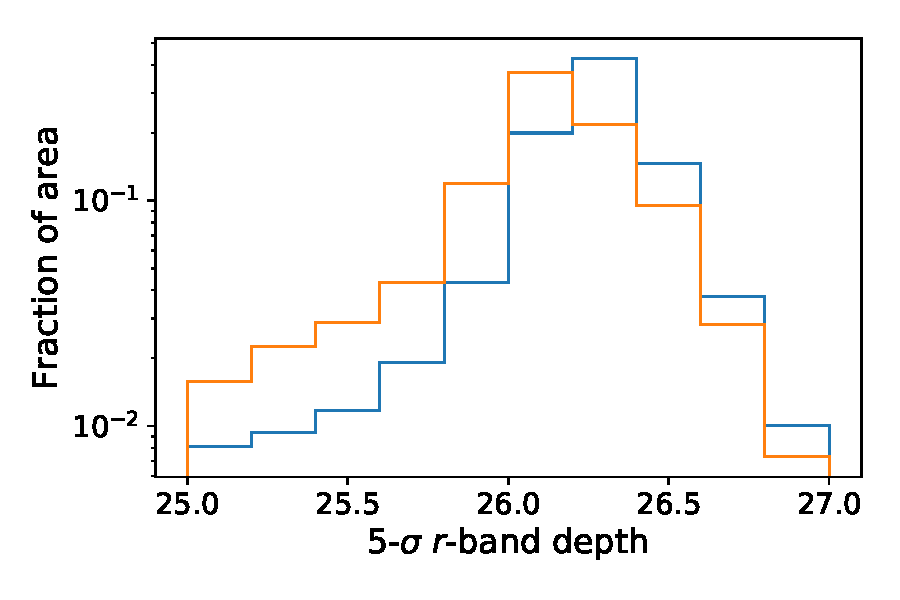
\includegraphics[width=0.85\columnwidth]{depth_comparison_1d.pdf}
\caption{5-$\sigma$ depth maps for the dithered (top) and undithered (middle) fields. There is an increased depth in the overlapping parts of the pointings in the undithered field but the median depth is lower. The maps have a resolution of $1.74$ arcmin. We also show the 1D distribution of depth (bottom) for both fields for easier comparison.}
\label{fig:depth_maps}
\end{figure}

We also check the depth by computing the detection efficiency (completeness\footnote{Note that a different completeness is defined in the star/galaxy classification section}) of stars and galaxies as a function of magnitude. To do so, we use the objects in the input catalog and select those that lie within the simulated footprint. After this, we compute the number of detected objects in the \textit{final sample} classified as stars and classified as galaxies as a function of their \texttt{CMODEL} magnitude, and divide by the number of stars and galaxies in the input catalog as a function of the true magnitude. The results can be seen in \figref{stellar_detection_efficiency}. We see that there is a high detection efficiency $> 80\%$ up to $r \approx 25.5$.  

\begin{figure}
\centering
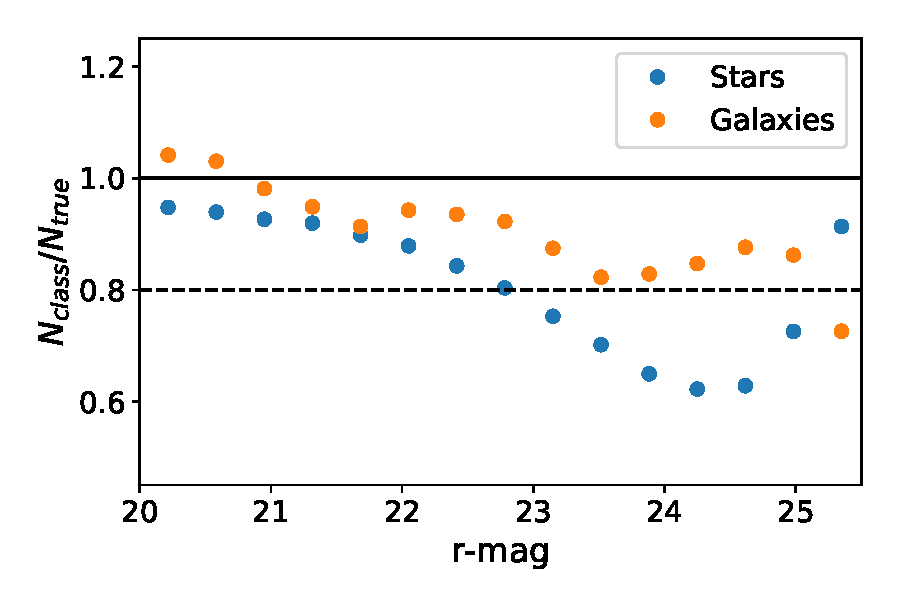
\includegraphics[width=0.9\columnwidth]{stellar_detection_efficiency.pdf}
\caption{Ratio of number of objects in the final sample classified as stars and number of input stars as a function of magnitude. We also compute this same ratio for galaxies. This is basically a measurement of the detection efficiency (completeness) of stars and galaxies in the final sample. Note that the ratio can go above one since there will be stars classified as galaxies (and galaxies classified as stars) and artifacts that will pass our cleaning cuts.}
\label{fig:stellar_detection_efficiency}
\end{figure}

Given the results in the two previous subsections and this subsection, we decide to use only the galaxies that lie in cells with limiting magnitude $r \geq 25.5$ and that have been visited at least, 92 times, which corresponds to 50\% of the nominal full-depth number of visits~\citep{Overview}. On top of that, we select those objects with magnitude $20 \leq r \leq 25.5$. This cut ensures high detection efficiency ($>80\%$) and it allows us to eliminate most of the artifacts in the sample. In addition it results in a low stellar contamination ($f_{star} \approx 1.4\%$). After these cuts and selecting objects with extendedness=1, we obtain 4.5 and 4.0 million objects for the dithered and undithered fields respectively. This selection cut however, does not change the fraction of unmatched objects explored in the previous subsection.

\subsection{Bright star masking}

Bright objects produce significant effects in the image that affect the detection and measurement of neighboring objects. Some examples of these effects include saturation, large diffraction spikes (not included in our simulations), scattered light (also not included in our simulations), obscuration of neighboring sources, etc. Thus, masking a region around these sources creates a more complicated footprint but greatly simplifies the analysis of systematic effects. In order to avoid possible biases by masking bright galaxies we will only analyze the impact of bright stars in the nearby detected objects. In the following, when we refer to bright object masking we are actually referring to bright star masking.

In order to evaluate the effect of bright star masking, we follow the procedure described in \citet{2018PASJ...70S...7C}. Using the position of bright objects classified as stars (\texttt{base\_ClassificationExtendedness\_value==0}), that lie within the considered footprint, and with input magnitudes in the range $m_{1} < r < m_{2}$ we count all objects from the final sample in a given radius $\theta$, and compute the mean of the set, $N_{neighbors}$. We repeat this for different radii and magnitude ranges ($ r < 17; 17 \leq r < 18; 18 \leq r < 20; 20 \leq r < 22$). Finally, we repeat this process for all stars in the input catalog in the footprint and compute $N_{neighbors, tot}$ and compute the ratio $N_{neighbors}/N_{neighbors, tot}$. Following \citet{2018PASJ...70S...7C} we use the point where the density reaches 95\% as masking radius. After this, we compare to equation (1) in \citet{2018PASJ...70S..25M}:
\begin{equation}
r_{mask,HSC} [\mathrm{arcsec}]= 200\times 10^{0.25(7-m_{B*})} + 12 \times 10^{0.05(16-m_{B*})}.
\end{equation}
Where $m_{B*}$ is the measured magnitude of the bright star to mask. Note that this prescription is specific for HSC. However, the LSST instrument and observing conditions are different. This is why we decided to rescale $r_{mask,HSC}$ by the ratio of mean seeing in LSST and HSC.
\begin{equation}
r_{mask,LSST} = r_{mask,HSC} \frac{1.04\arcsec}{0.58\arcsec}.
\end{equation}
Where 1.04\arcsec is the mean seeing in DC1, and 0.58\arcsec~is the mean seeing reported in~\citet{2018PASJ...70S..25M}. We obtain the results depicted in \figref{bright_object_masking}. We find that the masking radius, $r_{mask,LSST}$, using the rescaled prescription set by \citet{2018PASJ...70S..25M} is a pretty good approximation for our data. In particular, we find the ratio $r_{mask,fit}/r_{mask,LSST} \approx 1.14$. This 14\% disagreement can be related to the fact that we chose a very simple rescaling based on the mean seeing and due to our simplistic PSF model. As a result, we decide to use $r_{mask, DC1} = 1.14 r_{mask, LSST}$ around stars with $r < 22$. We generate a high-resolution mask using flat-sky maps of $\approx 6.4 \arcsec$ resolution, then we downsample this map to a resolution of $\approx 2$ arcmin and eliminate objects that lie within pixels that have more than 75\% of their area masked. This results in an area loss of $\approx 13\%$. The resulting map can be seen in \figref{bo_mask}. 
\begin{figure}
\centering
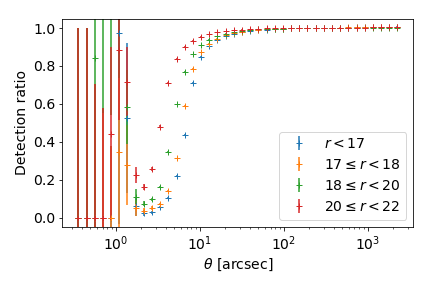
\includegraphics[width=0.9\columnwidth]{bright_object_masking}
\caption{Ratio of the median number of primary detected objects neighboring a star in a certain magnitude range in the input catalog to the median number of objects detected any star in the input catalog, as a function of the distance to the star $\theta$. Different colors represent different magnitude ranges for the stars in the input catalog considered.}
\label{fig:bright_object_masking}
\end{figure}
\begin{figure}
\centering
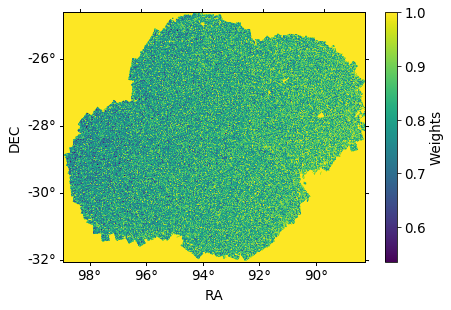
\includegraphics[width=0.9\columnwidth]{bo_mask}
\caption{Bright object (bright star) map. This map shows the unmasked fraction in each pixel. We use a high-resolution ($\approx 6.4 \arcsec$) map to mask around bright stars ($r < 22$) and then, we downsample the map to a lower resolution ($\approx 1.7 \arcmin$) and get rid of the pixels where the masked area by bright stars is higher than 75\% of the pixel.}
\label{fig:bo_mask}
\end{figure} 

%\subsection{Sample purity and effect of unmatched sources}
%Now, we have a robust sample (final sample). However, even after all our selection cuts, there are still a fraction of objects ($\approx 3\%$) that remain without a match in the input catalog. A reasonable question to ask now is: ``What is the nature of these unmatched objects?" and ``how much do these affect to a cosmological analysis?". In order to answer these questions, we estimate the power-spectra of the match and unmatched sources in the final sample as an ensemble ($C_{\ell}^{\rm{final}}$) and separately ($C_{\ell}^{\rm{matched}}, C_{\ell}^{\rm{unmatched}}$) and compare the results using a $\chi^{2}$ metric defined as: 
%\begin{equation}
%\tilde{\chi}^{2} = \sum_{\ell,\ell^{\prime}} \left(C_{\ell}^{\rm{final}}-C_{\ell}^{\rm{matched}}\right) \mathcal{C}_{\ell, \ell^{\prime}}^{-1}  \left(C_{\ell^{\prime}}^{\rm{final}}-C_{\ell^{\prime}}^{\rm{matched}}\right)
%\end{equation} 
%Where $\mathcal{C}_{\ell,\ell^{\prime}}$ is the covariance matrix. The details about how the power-spectra and their covariances are computed are described in Section~\ref{sec:results}. The results of this comparison can be seen in \figref{cl_matched_unmatched}. We see that the unmatched objects have a very different nature and power-spectrum that the matched objects. These objects are mostly bright sources split into smaller sources, noisy pixels identified as sources, or mischaracterized heavily blended sources. We show that, given our area, we are have a close to 2-$\sigma$ difference between the matched objects in the final sample and the ensemble since the total $\tilde{\chi^{2}}=21$ with 16 degrees of freedom. We can see that the greatest differences start from $\ell > 2000$ where shot-noise starts to be dominant and the correction for the shot noise that we perform $1/n$, where $n$ is the number density, may be no longer valid. However, if we were to consider a footprint such as the expected LSST Y10 area given by the DESC SRD~\citep{2018arXiv180901669T} of 14,300 deg$^{2}$, this would mean that our total $\tilde{\chi^{2}} \approx 9250$ which means that these unmatched objects make a very significant difference, when considering the full LSST area, highlighting the sensitivity of LSST. For this study we could have required to have a match in the input catalog to remain in the final sample, however, we decided to mimic the analysis of real data where we will not have a truth catalog available. The measurements in more filters/bands will provide us with additional criteria to clean the sample, and reduce the incidence of possible artifacts but follow-up studies should be performed in future data challenges in order to provide robust criteria to filter potential artifacts in multi-band LSST data.
%\begin{figure}
%\centering
%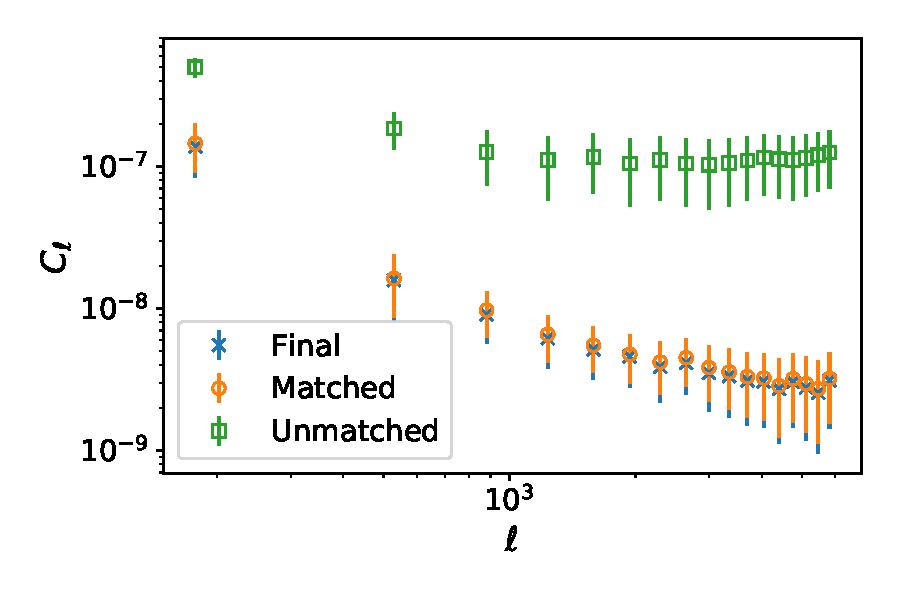
\includegraphics[width=0.9\columnwidth]{cl_matched_unmatched}
%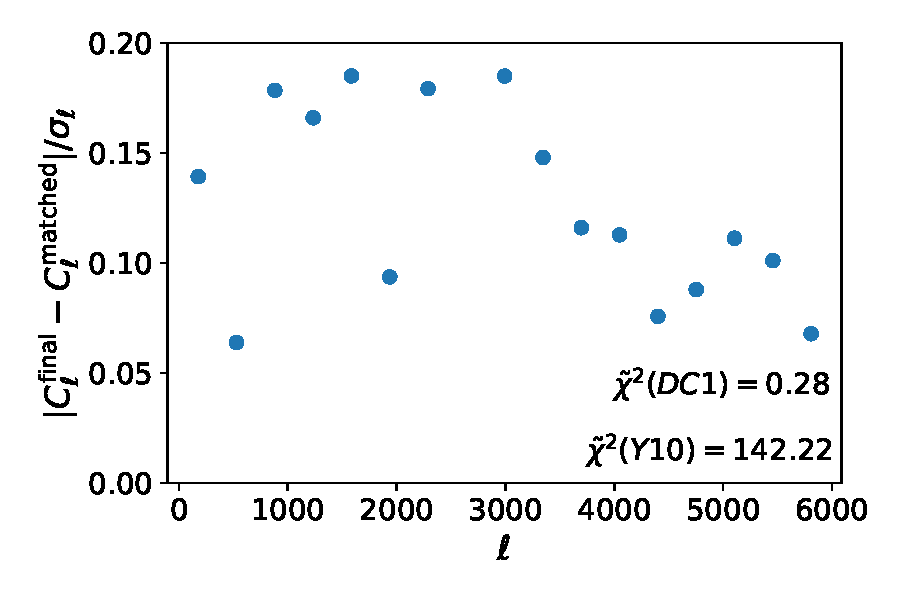
\includegraphics[width=0.9\columnwidth]{cl_chi2_mu}
%\caption{\textbf{Top panel:} Angular power-spectra of the matched sample and unmatched sample. \textbf{Bottom panel:} Relative difference of the matched power-spectrum and the final sample power-spectrum compared to the statistical uncertainty. We see that the difference for DC1 is not statistically significant. Error-bars are computed using the Gaussian covariance matrix in \texttt{NaMaster}.}
%\label{fig:cl_matched_unmatched}
%\end{figure}

\subsection{Blending}
As previously mentioned, our output catalogs do not include any estimation of overlap between sources, or \textit{blendedness}~\citep{2018PASJ...70S...5B}. Highly-blended objects are more likely to have biased estimations of the centroid position, shape, and fluxes. This can lead to overall biases in the estimated photometric redshifts and cosmological parameters. Given that the mean seeing in DC1 is larger than in HSC, the impact of blended objects will be larger. In the case of \citet{2018PASJ...70S..25M}, the cut in the blendedness parameter affects only 1\% of the objects; we expect this number to be larger in our case. Using specialized image simulations from~\citet{Sanchez19} with a seeing similar to the seeing in DC1 (1.04\arcsec), in $r$-band, we find that if we select objects with $r < 25.5$ and SNR $\geq 1$, the fraction of objects with blendedness $ >10^{-0.375}$ is $\approx 6.3\%$. If we raise the minimum SNR threshold to 6, this fraction is lowered to $\approx 2.6\%$. This means that our sample will have a fraction of these objects anywhere in the range (2.6\% - 6.3\%) but closer to 2.6\% since the fraction of objects with SNR $\leq 6$ is $\approx 0.3\%$. In any case, we do not expect that the inclusion of these objects in our two point measurements will affect the range of scales that we are going to consider in this work. A more rigorous study of the impact of blending on small-scale clustering measurements is beyond the scope of the current work.


%%% Commenting out the 2pt results section %%%
% -------------------------------------------------------------------%
%\iffalse
%%%%
\section{Two-point clustering results}
\label{sec:results}

In this section, we analyze the two-point clustering statistics for the DC1 dithered and undithered catalogs. This analysis serves as validation for our simulated data and our clustering analysis pipeline, and it also allows us to study the impact of the dither strategy in the mitigation of systematics.

In particular, we are going to consider maps of the following observational effects:
\begin{itemize}
\item Extinction: The CatSim catalog provides the value for the magnitudes corrected for extinction using the map from \citet{1998ApJ...500..525S}, which we refer to as the SFD map.
\item Stellar contamination: In this case, we build a flat-sky map with all stars in the input catalog.
\item Sky-background/Sky-brightness: We use the observed background level in each exposure and assign that value to the pixels in the flat-sky map that lie within that exposure. After this we calculate the mean value in each pixel to build the map with the same resolution as the mask ($\approx 2$ arcmin) which we deproject~\citep{2019MNRAS.484.4127A}. 
\item Sky-noise: We use the observed noise background level in each exposure and proceed as in the previous case to build a map.
\item Seeing: We proceed as before and use the observed seeing in each exposure and build a map.
\item Number of visits: We count the number of exposures overlapping with each pixel of our flat-sky maps.
\end{itemize}
These maps are shown in \figref{systematic_maps} and \figref{systematic_maps_ud}. We see that the spatial distribution of the different observing conditions are very different between the two simulations, even though the ranges in each of the observing conditions are very similar. 

\begin{figure*}
\centering
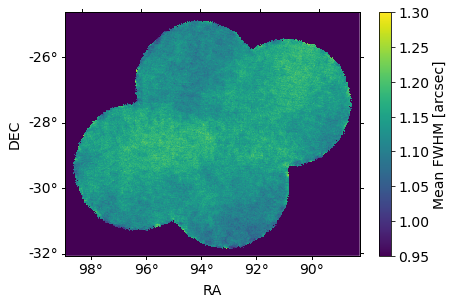
\includegraphics[width=0.30\textwidth]{mean_fwhm.png}
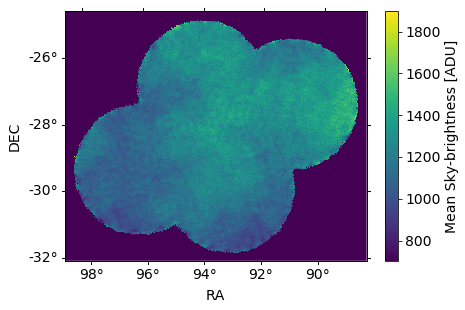
\includegraphics[width=0.30\textwidth]{mean_sky.png}
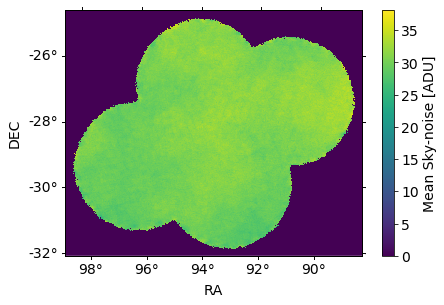
\includegraphics[width=0.30\textwidth]{mean_skynoise.png}
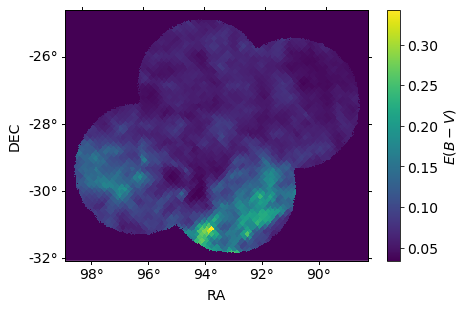
\includegraphics[width=0.30\textwidth]{extinction.png}
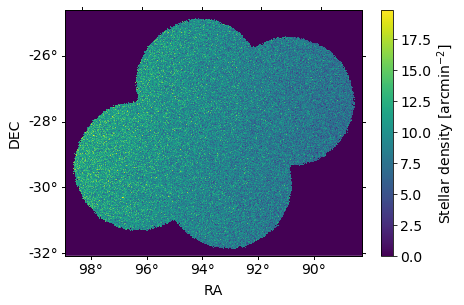
\includegraphics[width=0.30\textwidth]{stellar_density.png}
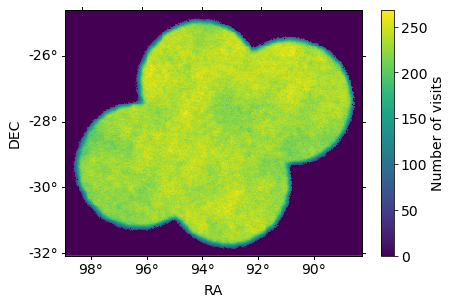
\includegraphics[width=0.30\textwidth]{nvisits.png}
\caption{Maps showing the different foregrounds considered in our analysis of the dithered field. From top left to bottom right: Mean PSF FWHM, mean sky-brightness, mean sky-noise, mean extinction, stellar density and number of visits in each pixel in the flat-sky maps with the same resolution as the depth maps in \figref{depth_maps}. We only show their values in the regions where the 5-$\sigma$ $r$-band depth is larger than 25.5.}
\label{fig:systematic_maps}
\end{figure*}

\begin{figure*}
\centering
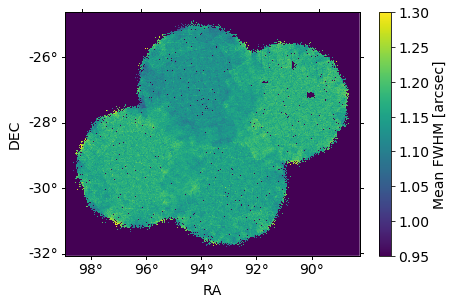
\includegraphics[width=0.30\textwidth]{ud_mean_fwhm.png}
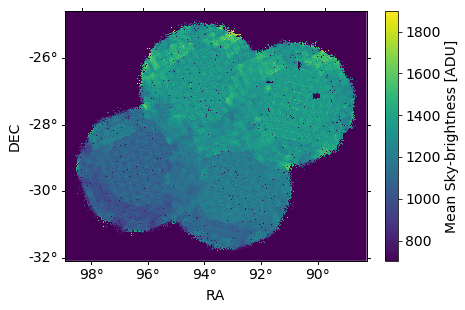
\includegraphics[width=0.30\textwidth]{ud_mean_sky.png}\\
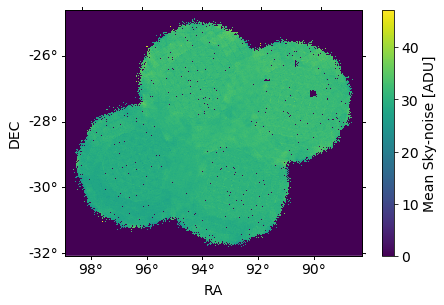
\includegraphics[width=0.30\textwidth]{ud_mean_skynoise.png}
%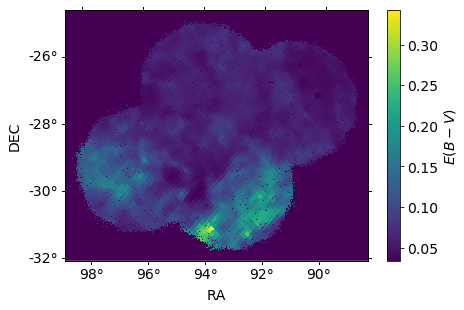
\includegraphics[width=0.40\textwidth]{ud_extinction.png}
%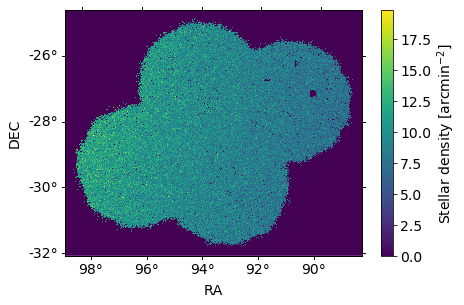
\includegraphics[width=0.40\textwidth]{ud_stellar_density.png}
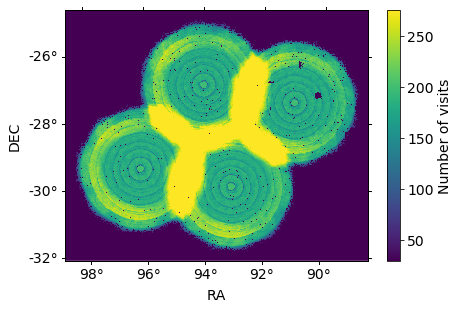
\includegraphics[width=0.30\textwidth]{ud_nvisits.png}
\caption{Same as \figref{systematic_maps} for the undithered dataset. From top left to bottom right: Mean PSF FWHM, mean sky brightness, mean sky noise and number of visits. Note that we use the same extinction and stellar density maps changing the geometry of the mask.}
\label{fig:systematic_maps_ud}
\end{figure*}

The power-spectra computation and correction for the effect of systematics is performed using NaMaster~\citep{2019MNRAS.484.4127A}. The systematics correction is also performed with NaMaster via mode deprojection, which assumes that there is a linear dependence between the observed number density of galaxies and the contaminants. For our study, we choose $\Delta \ell = 352$ and compute the power-spectra in the range $0 \leq \ell \leq 6000$. This choice for $\Delta\ell$ is not optimal for cosmological analyses, but it gives us a reasonably large number of bandpowers to visually check the estimated power-spectra. The results for the power-spectra are shown in~\figref{power_spectra}, where we can see that both the dithered and undithered catalogs yield similar results. The error-bars shown and corresponding covariances are estimated using two complementary methods: On the one hand by computing the Gaussian covariance with NaMaster, and on the other hand by considering 155 jackknife equal area regions in our footprint. We find both approaches to give similar results and we choose to use the results from the jackknife computation.
\begin{figure}
\centering
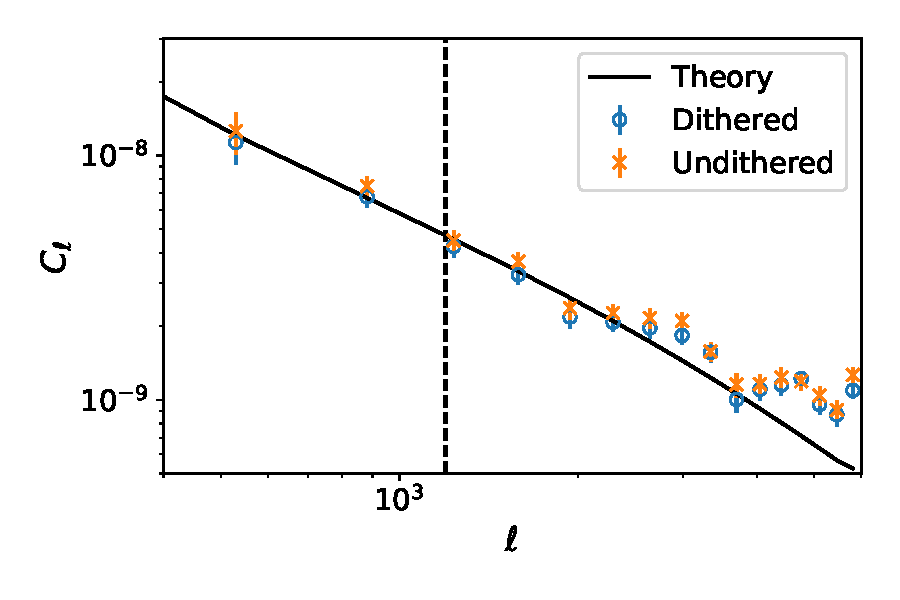
\includegraphics[width=0.9\columnwidth]{Cl_results_2019_comp}
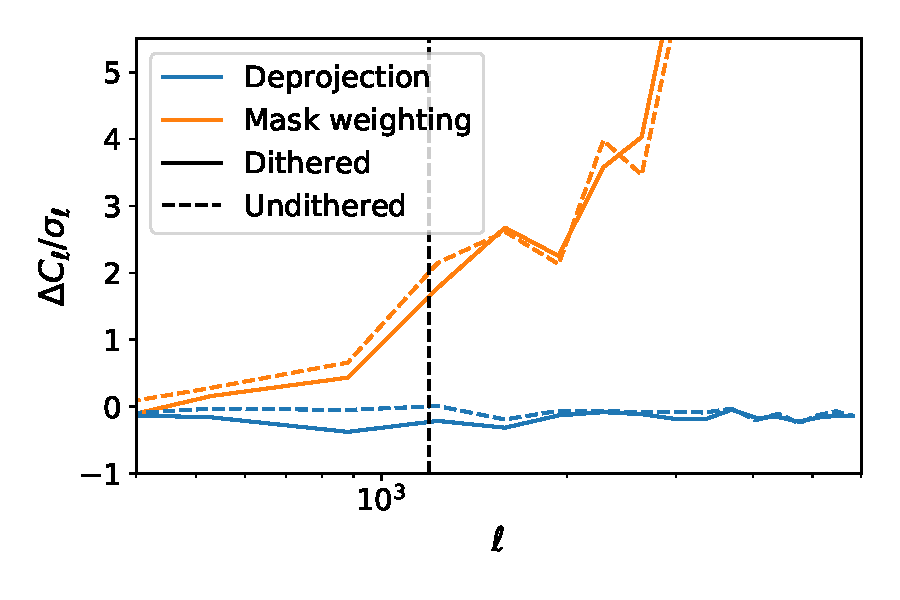
\includegraphics[width=0.9\columnwidth]{systematics_comp_abs}
\caption{{\bf Top panel:} Measured power spectra undithered (orange $\times$) and dithered (open blue circles) datasets with NaMaster corrected by systematics. The error bars are computed using jackknife. A theoretical prediction is shown as the solid black line to demonstrate the overall agreement between the measurements and the data. The vertical black dashed line corresponds to $\ell = 1/f_{sky}=1192$ ($k \sim 0.9$ Mpc$^{-1}$ at the mean redshift of the final sample $\bar{z} \approx 1.51$). {\bf Bottom panel:} Size of the correction in the power-spectra, $\Delta C_{\ell}$, relative to their uncertainty, $\sigma_{\ell}$, due to deprojection (blue) of different observing conditions, and the correction due to weighting by the bright object mask (orange) for the dithered (solid lines) and undithered (broken lines) simulations. We see that the largest impact comes from the presence of bright objects, and that it is important to account for the area lost by masking via weighting. The horizontal dashed line corresponds to a correction of 50\% of the statistical uncertainty to provide visual guidance.} 
\label{fig:power_spectra}
\end{figure}

%\begin{figure}
%\centering
%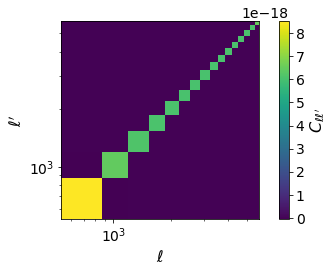
\includegraphics[width=0.9\columnwidth]{Gaussian_covariance}
%\caption{Estimated Gaussian covariance using \texttt{NaMaster} in the range of scales considered in our analysis.}
%\label{fig:gaussian_cov}
%\end{figure}
In this figure we also compare with the theoretical prediction for the power-spectra computed with \texttt{CCL}~\citep{2019ApJS..242....2C} as follows:
\begin{equation}
C_{\ell}^{\rm TH} = \frac{2}{\pi}\int{dz} \left(\frac{dn(z)}{dz}\right)^{2} b^{2}(z) \int{dk k^{2} P(k,z)j^{2}_{\ell}(kr(z))},
\end{equation}
where $P(k,z)$ is the power spectrum, $b(z)$ is the galaxy bias and $\frac{dn}{dz}$ is the number density as a function of redshift. In particular, we use the Halofit~\citep{2012ApJ...761..152T} power-spectrum with the Millenium cosmological parameters~\citep{2005Nature.435.629S} ($\Omega_{m}=0.25$, $\Omega_{b}=0.045$, $\Omega_{\Lambda}=0.75$, $n=1$, $\sigma_{8}=0.9$, $h=0.73$), and the $dn/dz$ obtained using the true redshifts of galaxies matched in the input catalog. We use a bias, $b(z) = b_{0}/D_{+}(z)$, inversely proportional to the linear growth factor, $D_{+}(z)$, and see that, qualitatively speaking, there is a good agreement between the measurements and the prediction, as shown in~\figref{power_spectra}. %The best-fit value that we find for $b_{0}=0.45$. This low value for the galaxy bias is a consequence of the addition of non-clustered galaxies at the fainter end ($r > 25$) in order to match the expected number density for LSST (Connolly private comm.). 
However, we do not expect to be able to fully describe the measured power-spectra, given the highly-nonlinear nature of the scales considered in our analysis.

In addition, we also see in~\figref{power_spectra} that the overall impact of the systematics is smaller than statistical uncertainty, $\sigma_{\ell}$, (about 50\% the size of $\sigma_{\ell}$) and that they similarly affect both dithered and undithered simulations. We do not find any statistically significant difference between the correction due to systematics for the dithered and undithered simulations. This is a consequence of several factors, including the conservative cuts that we impose on our data to ensure well-behaved clustering statistics; that we only deproject using the mean value for the different observing conditions; and the lack of effects, such as vignetting, present in real images. For example, vignetting would affect the number of detected objects close to the edges of the focal plane in the undithered simulation, reducing the uniformity of the survey. However, this effect would be uniform across the footprint in the dithered case. In addition to this, if we decided to push our data further by going deeper, the systematic lack of uniformity of the undithered field would start to play a large role in the impact of the observing conditions over the clustering signal. We can also see that, in the $\ell$ range considered in our analysis, the presence of bright objects -- in particular bright stars -- is the dominant systematic effect. In the close neighborhood to bright objects our ability to detect faint sources diminishes. These faint sources are blended in the core or the tails of the brighter objects, resulting in a lower mean number of detected sources, as shown in \figref{bright_object_masking}. The correction due to weighting by the fraction of area covered in each pixel has a considerable impact at small-scales, being larger than the statistical uncertainty in this regime. This showcases again the importance of considering the impact of blending in the small-scale regime for LSST and should be carefully studied in future Data Challenges. The correction due to the presence of bright objects is comparable in both simulations. We expect that for future versions of the LSST Science Pipelines this effect will be smaller due to improvements in the deblending and measurement algorithms.


\section{Conclusions}
\label{sec:conclusions}

End-to-end simulations are powerful tools for testing the overall performance of current and future cosmological experiments like the LSST. They allow us to validate and improve various aspects of the the data processing and analysis, as well as to model and improve our control of systematic uncertainties. The access to ground truth allows us to test certain aspects of the processing and analysis pipelines that would be otherwise very challenging to test with real data (e.g., impact of undetected sources in the fluxes of detected overlapping sources). Realistic and validated synthetic datasets will be required for successful control of systematics.

In this paper, we present an end-to-end simulated imaging dataset that resembles single-band, full-depth (10-year) LSST data (for the wide-fast-deep survey), for the first data challenge, DC1, in the LSST DESC. This dataset was generated by synthesizing sources from cosmological N-body simulations in individual sensor-visit images with different observing conditions. Two separate runs of this dataset were generated with different dither strategies, the dithered run and the undithered run. The images from both runs were processed with the LSST Science Pipelines (DM stack). We perform several quality assurance tests on the resulting data product, including all of the LSST Science Requirements~\citep{LPM-17} Key Performance Metrics and the DESC Science Requirements~\citep{2018arXiv180901669T} testable with DC1. Both datasets successfully pass these tests.

We study different ways to relate the output catalogs to the inputs: The first method uses information about positions only, and the second involves both positions and magnitudes. For clustering analyses, adding information about magnitudes results in a lower incidence of spurious matches and is sufficient for DC1, however, none of these methods provide a noiseless match between inputs and outputs. We also realize that these matching techniques are likely insufficient for studies on blending or scales smaller than those considered in this work, since they do not include information about undetected sources present in blends. Therefore, an important research topic for these kinds of end-to-end simulations is to find efficient strategies to relate inputs and outputs. 

The usage of matching strategies helps us define a final sample suitable for clustering analyses. After cleaning the catalog, we find a small fraction ($\approx 3.6\%$) of artifacts, i.e., objects with no counterpart in the input. We demonstrated that our selection criteria is robust given the DC1 area. However, careful data-selection criteria will be needed to enable accurate clustering analyses for the larger Y10 dataset. We anticipate that additional information coming from multi-band coverage and photometric redshifts, will help us to further refine the selection.

We use our final sample to perform clustering analysis. The results of this analysis indicate that the simulated contaminants have a low impact, smaller than the statistical uncertainty, in both datasets. This is probably due to the simplicity of our foregrounds, and more complexity will be added in future data challenges. We do not find statistically significant differences in the impact of systematics between the dithered and undithered datasets given the area of DC1. We also see that, in the aforementioned scale-range, the presence of bright objects has a larger impact on the power-spectra, $\approx 200-600\%$ of the statistical uncertainty, highlighting the impact of blending in LSST for small-scale analyses.

Finally, we have been able to perform an end-to-end test of our processing and analysis pipelines, which will enable a better exploitation of future LSST data. The methodology presented in this work will serve as the basis for future DESC data challenges, where we aim to perform multi-band studies in a larger area, analyze complementary image generation strategies (PhoSim), and increase the complexity of the foregrounds included.

% ----------------------------------------------------------------------
\appendix
%\section{Detailed astrometric and photometric tests}

%We show the detailed astrometric repeatability in \figref{validate_drp_check_astrometry}, where detected stars that are detected at different visits are matched and their astrometric residual is shown as a function of their SNR.

%\begin{figure}
%\centering
%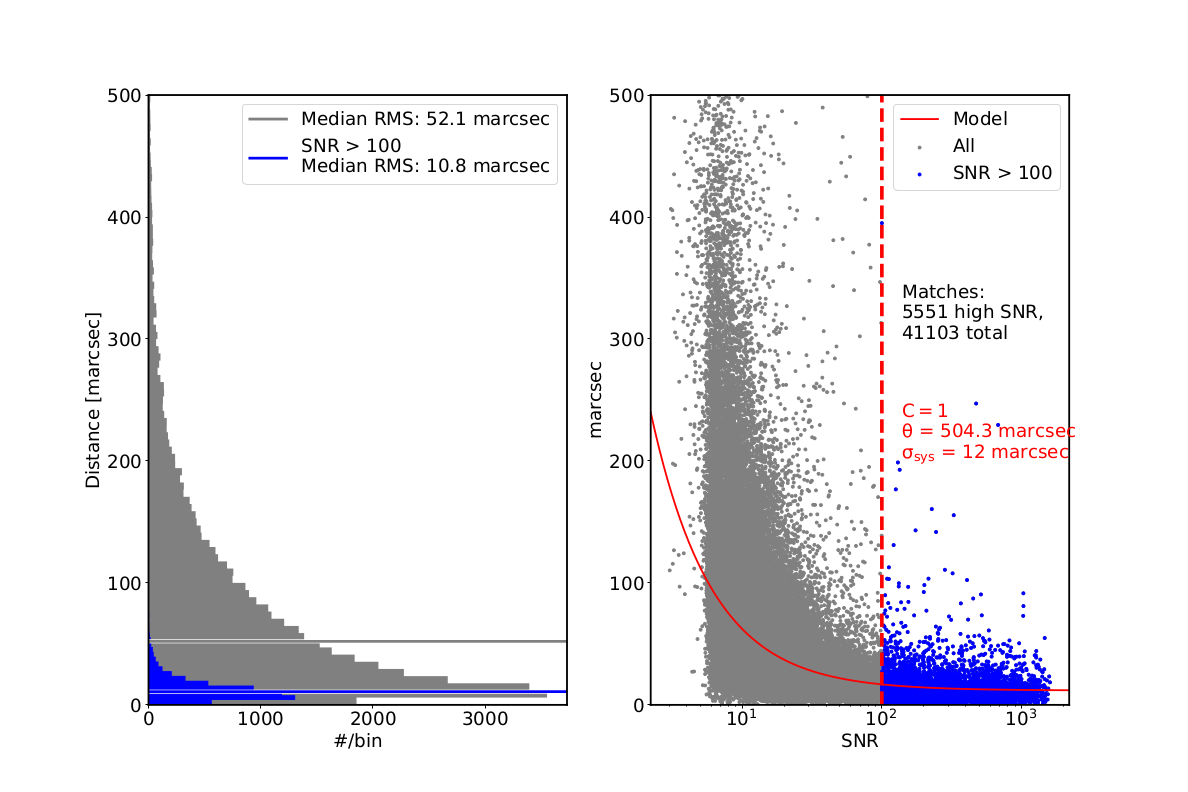
\includegraphics[width=0.9\columnwidth]{DC1-imsim-dithered_r_check_astrometry.png}
%\caption{
%Detailed astrometric performance.  (left) Histogram of the repeatability of distance between pairs of stars.  (right) Astrometric variation as a function of SNR.  We find a systematic floor of 12~milliarcsec.
%}
% MWV: A good thing to think about someday, but not necessary for this paper:
% {\bf TODO: MWV IS THIS HISTOGRAM DIFFERENT THAN THE check\_photometry histogram in terms of per-pair vs. per-object variation.}}
%\label{fig:validate_drp_check_astrometry}
%\end{figure}

\section{LSST SRD requirements}
\label{app:lsst_srd}
In this section we are going to summarize the different requirements that we test for from the LSST Science Requirements Document version 11 that can be found at \url{https://docushare.lsst.org/docushare/dsweb/Get/LPM-17}.

\subsection{General requirements}
\begin{itemize}
\item Nv1: Minimum number of visits in a given filter. It should be at least 184 for r-band
\item pixSize: Maximum pixel size. The pixel size should be smaller than 0.22 arcseconds.
\end{itemize}

\subsection{Astrometric requirements}
\begin{itemize}
\item AA1: Astrometric accuracy check. Minimum absolute astrometric accuracy. We compute it as the median of the difference between input and measured centroid positions. The maximum median value is 100 milliarcseconds.
\item AMx: Astrometric repeatability check. Maximum RMS of the separation between pairs of stars separated by 5 arcmin (AM1: 20 milliarcseconds), 20 arcmin (AM2: 20 milliarcseconds), and 200 arcmin (AM3: 30 milliarcseconds). 
\item AFx: Astrometric repeatability check. Maximum outlier fraction that deviate more than 40 mas (50 mas for AF3) for the separation between pairs of stars separated by 5 arcmin (AF1: 20 \%), 20 arcmin (AF2: 20\%), and 200 arcmin (AF3: 20\%).
\end{itemize} 

\subsection{Photometric requirements}
\begin{itemize}
\item PA1: Photometric repeatability check. Maximum RMS/IQR of the magnitude distribution of objects between different visits. The maximum value allowed is 8 millimags.
\item PF1: Photometric repeatability check. Maximum outlier fraction that deviate more than 15 millimag (PA2) from the mean measured magnitude. The value for this requirement is 20\%. 
\item PA6: Photometric accuracy check. Minimum absolute photometric accuracy. We compute this as the median difference between the input and measured fluxes for stars. The maximum value allowed is 20 millimag.
\end{itemize}

\subsection{Zeropoint uniformity requirements}
\begin{itemize}
\item PA3: Zeropoint error uniformity. Maximum allowed value for the RMS of the photometric zeropoint error. The value for this requirement is 15 millimags.
\item PF2: Zeropoint error uniformity. Maximum outlier fraction that deviate more than 15 millimag (PA4) in the zeropoint error distribution. The value for this requirement is 10\%
\end{itemize}

\subsection{Depth requirements}
\begin{itemize}
\item D1: Minimum depth check. Minimum value for the median of the 5$\sigma$ $r$-band depth for single visits with seeing 0.7 arcseconds, airmass 1.0 and 30 seconds exposure time. The value for this requirement is 24.3.
\item Z1: Minimum depth check. Minimum value for the 20-th percentile (DF1) of the 5-$\sigma$ $r$-band depth distribution for single-visits with seeing 0.7 arcseconds, airmass 1.0, skybrightness fainter than 21 in $r$-band, and 30 seconds exposure time.
\item DB1: Minimum depth check. DB1 is effectively the same requirement as D1, generalized to other bands (in the case of DC1 it is exactly the same as D1).
\item Z2: Minimum depth check. Maximum variation within the field-of-view for the brightest 20-th percentile (DF2) of the depth in a representative single visit. The value for this requirement is 0.4.
\end{itemize}

\subsection{Image quality requirements}
\begin{itemize}

\item SE1: Maximum PSF ellipticity check. Maximum median value of the PSF ellipticity modulus. The value for this requirement is 0.05.
\item SE2: Maximum PSF ellipticity check. Maximum value for the 90th percentile (EF1) of the PSF ellipticity modulus. The value for this requirement is 0.1.
\item SRx: Image quality test. Minimum radii to encircle at least 80\% (SR1), 95\% (SR2), and 99\% (SR3) of the energy for a fiducial delivered seeing of 0.69 arcseconds. The values are 0.80, 1.31, and 1.81 arcseconds for SR1, SR2, and SR3 respectively.
\item TE1: PSF ellipticity residual correlation check. Maximum value for the median PSF ellipticity correlations $E_{1}, E_{2}, E_{3}$ defined in equations (8-10) for $\theta \leq 1$ arcmin. The value for this requirement is $3 \times 10^{-5}$.
\item TE2: PSF ellipticity residual correlation check. Same as TE1 but for $\theta \geq 5$ arcmin. The value for this requirement is $2 \times 10^{-7}$. 
\end{itemize}
\subsection*{Acknowledgments}
This paper has undergone internal review in the LSST Dark Energy Science Collaboration. The internal reviewers were Andrina Nicola, Alex Drlica-Wagner and Nacho Sevilla.
FJS thanks Amanda Pagul, David Alonso. This research used resources of the National Energy Research Scientific Computing Center, a DOE Office of Science User Facility supported by the Office of Science of the U.S. Department of Energy under Contract No. DE-AC02-05CH11231. We acknowledge the use of \texttt{Pandas, Dask, SciPy, Matplotlib, Jupyter, CCL, NaMaster, Healpy, and scikit-learn} as well as the LSST software stack.
The work of FJS and DK was supported by the US Department of Energy award DE-SC0009920. The work of CWW was supported by the US Department of Energy High Energy Physics grant DE-SC0010007. The work of JC, RD, SD, TG, AJ, HK, PJM and BVK was supported by the U.S. Department of Energy under contract number DE-AC02-76SF00515. The work of RM was supported by the US Department of Energy Cosmic Frontier progam, grant DE-SC0010118. 


%
The DESC acknowledges ongoing support from the Institut National de Physique Nucl\'eaire et de Physique des Particules in France; the Science \& Technology Facilities Council in the United Kingdom; and the Department of Energy, the National Science Foundation, and the LSST Corporation in the United States.  DESC uses resources of the IN2P3 Computing Center (CC-IN2P3--Lyon/Villeurbanne - France) funded by the Centre National de la Recherche Scientifique; the National Energy Research Scientific Computing Center, a DOE Office of Science User Facility supported by the Office of Science of the U.S.\ Department of Energy under Contract No.\ DE-AC02-05CH11231; STFC DiRAC HPC Facilities, funded by UK BIS National E-infrastructure capital grants; and the UK particle physics grid, supported by the GridPP Collaboration.  This work was performed in part under DOE Contract DE-AC02-76SF00515.
This manuscript has been authored by Fermi Research Alliance, LLC under Contract No. DE-AC02-07CH11359 with the U.S. Department of Energy, Office of Science, Office of High Energy Physics.

% 


Author contributions are listed below. \\
J.~S\'{a}nchez: led study \\
C.~W.Walter: led image generation \\
A.~Slosar: Participated in analysis and preliminary tests \\
D.~Kirkby: Participated and advised in analysis \\
J.~Chiang: One of the main developers of imSim, participated in image generation and data distribution \\
T.~Glanzman: Generated artificial images \\
S.~F.~Daniel: Developed imSim and CatSim \\
H.~Awan: Participated in analysis and designed dithering strategy \\
E.~Gawiser: Participated in analysis and designed dithering strategy \\
W.~M.~Wood-Vasey: Ran validation software and wrote part of the document \\
Y.~AlSayyad: LSST Science Pipelines \\
%C.~Burke: Contributions to PhoSim \\
%J.~Cheng: Contributions to PhoSim \\
S.~Digel: Workflow and validation \\
%R.~Dubois: Workflow and management \\
%M.~Jarvis: Contributions to imSim and validation \\
T.~Johnson: Workflow, data generation and processing \\
H.~Kelly: DMstack librarian at NERSC \\
S.~Krughoff: Contributions to LSST Science Pipelines and DC1 workflow \\
R.~H.~Lupton: LSST Science Pipelines, overall QA \\
R.~Mandelbaum: Provided feedback on DC1 design, analysis, and paper draft \\
P.~J.~Marshall: Led the ``Twinkles'' DC1 pathfinder project. \\
%M.~Mustafa: NERSC workflow \\
%E.~-H.~Peng: Contributions to PhoSim \\
J.~R.~Peterson: PhoSim Development for DC1 \\
%P.~Price: LSST Science Pipelines \\
%G.~Sembroski: PhoSim Development for DC1 \\
%B.~Van Klaveren: DC1 workflow \\
M. P.~Wiesner: Completed a study on astrometry in PhoSim making it possible to improve astrometry in PhoSim for DC1 \\
B.~Xin: Contributions to ImSim and PhoSim \\


\bibliography{lsstdesc,main}

\end{document}


% ======================================================================
%
